% =====================================================================
% A Shared Valence Axis Across Modern LLMs and Human EEG: The Saturation Regularity
% ICLR 2027 anonymous submission
% =====================================================================

\documentclass{article}

% --- ICLR 2027 submission (anonymous / double-blind). ---
% Authors are hidden automatically in submission mode; for the camera-ready,
% place \iclrfinalcopy before \begin{document} to de-anonymize.
\usepackage{iclr2027_conference,times}

% === Core packages ===
\usepackage[utf8]{inputenc}
\usepackage[T1]{fontenc}
\usepackage{amsmath}
\usepackage{amssymb}
\usepackage{amsfonts}
\usepackage{graphicx}
\usepackage{booktabs}
\usepackage{url}
\usepackage{microtype}
\usepackage{xcolor}
\usepackage{hyperref}
\usepackage{xspace}
\usepackage{caption}
\usepackage{subcaption}
\usepackage{multirow}
\usepackage{nicefrac}
\usepackage{enumitem}


\graphicspath{{figures/}}

% === Cross-referencing ===
\usepackage[capitalize,noabbrev]{cleveref}
\title{The Saturation Regularity: When Concept-Aligned Supervision Stops Helping Converged EEG Classifiers}

\author{Anonymous Authors}

\begin{document}

\maketitle

\begin{abstract}
A common machine-learning technique adds an \emph{auxiliary loss}
that pushes a network's internal features toward a known target
direction in feature space---for example, the difference between
positive and negative sentiment, or between calming and disturbing
emotion. We test $25$ such recipes (knowledge distillation,
representational-similarity analysis, contrastive losses, low-rank
adapters, channel-targeted brain-region losses) on
FACED~\citep{chen2023faced}, a public dataset of EEG recordings from
$123$ subjects watching $28$ emotional video clips, with $9$ emotion
classes. None help: $16$ of the $25$ produce statistically significant
accuracy decrements, and $0$ produce gains. We trace this to a
regularity we call \emph{saturation}: once a network has converged on
the emotion classification task from labels alone, its features
already encode the target concept; the auxiliary loss then adds
gradient noise rather than information. Saturation is distinct from
overfitting (memorising the training set); it is a property of how
task and auxiliary supervision interact once both target the same
direction in feature space. The same picture suggests a positive
prescription: ensemble across the seed-specific differences in the
features, rather than supervise the part of the features that has
already saturated. Following this prescription on FACED yields a new
state of the art at $\mathbf{0.6948}$ balanced accuracy---a $+10.5\%$
relative improvement over EMOD~\citep{chen2025emod}, the previous SOTA
on FACED, at $0.6287$. Surprisingly, the language-model-derived class
prototypes used by the knowledge-distillation step in our recipe are
interchangeable with random orthonormal vectors ($\Delta\le 0.003$
balanced accuracy): the SOTA gain comes from the \emph{shape} of the
loss (a 9-class structure imposed on the features), not from the
\emph{content} of the prototypes. To probe what the network has
saturated on---and to demonstrate it is a real semantic axis, not a
noise dimension---we extract one direction explicitly. We write nine
short emotion-evocative stories (one per FACED class), pass them
through a language model (Qwen3-4B), and take the first principal
component of the language model's late-layer features across the nine
stories. We call this direction the \emph{valence axis}. The same
direction predicts movie-review sentiment zero-shot on
SST-2~\citep{socher2013recursive} at AUC $0.832$, predicts the EEG
response averaged across $123$ FACED subjects at $r=0.87$, and emerges
spontaneously in $36$ EEG classifiers trained only on the $9$ emotion
labels. All claims replicate on a second public EEG dataset,
SEED-V~\citep{liu2022seedv} (Appendix~\ref{app:seedv-full}).
\end{abstract}

\section{Introduction}
\label{sec:intro}

Auxiliary losses that pull a network's features toward a known concept
direction are a standard way to inject prior knowledge. We report a
regime in which they systematically backfire. Take an EEG emotion
classifier that has already converged, and add a loss aligning its
features with a valence direction: across twenty-five such recipes on
FACED~\citep{chen2023faced}, none improve balanced accuracy and fifteen
significantly reduce it. The same loss that helps a weak backbone hurts
a strong one. We call this the \emph{saturation regularity}: once task
labels alone have driven the network onto the target concept, further
supervision can only deform an already-converged representation, without
improving generalization. The finding is doubly useful. It explains a
widespread failure mode of concept-alignment supervision, and, by
locating where the recoverable gain does live---in the seed-specific
residual that supervision cannot exploit---it yields a new state of the
art through ensembling rather than supervising.

To make ``the concept the network has saturated on'' concrete, we
extract it explicitly. Pass nine short emotion-evocative sentences
through a language model, average the late-layer hidden states class by
class, and take the first principal component; the resulting
\emph{valence axis} (V-axis) predicts movie-review sentiment at AUC
$0.832$ zero-shot, tracks the cohort-averaged EEG response of $123$
subjects at the emotion-category level ($r{=}0.87$), and is rediscovered
without supervision by every reasonably-strong EEG classifier we tested.
Recent work shows that language models' internal features align with
human cognition across high-level
concepts~\citep{kim2018tcav,arditi2024refusal}; we use the V-axis as a
\emph{probe} of what brain-decoding networks encode, not as a training
signal---which, as the saturation regularity shows, a converged network
cannot benefit from.

\textbf{A nine-sentence axis.} The nine stories are one per
FACED~\citep{chen2023faced} class; the language model is Qwen3-4B,
chosen as the lead because it sits at the centre of the alignment
manifold in our $14$-LLM sweep, with the highest per-stimulus
alignment to a behavioural valence reference (the recipe itself is
model-agnostic, see Appendix~\ref{app:per-llm-deep-dive}). The SST-2
benchmark grounds the AUC $0.832$ headline:
the V-axis projection alone is within $0.005$ of a $5$k-example
supervised logistic regression~\citep{socher2013recursive}. And the
direction is not idiosyncratic to any one model: across the
$14$ language models from $560$M to $32$B parameters, the V-axis
converges on essentially the same direction (within Qwen3,
off-diagonal $r{=}{+}0.995$ over $15$ size-pairs).

\textbf{The same axis lives in the brain.} The $r{=}0.87$ above
unpacks as follows. A ridge regression on $160$ channel-band
features of the FACED cohort EEG predicts the V-axis position of
each of the $28$ stimuli; the regressor uses leave-one-stimulus-out
cross-validation, no per-subject fitting, no auxiliary supervision.
The Qwen3-4B V-axis itself reaches $r{=}0.80$ ($p<10^{-5}$) on this
ridge; a CLIP-text variant of the V-axis built from the same $28$
stimulus descriptions tightens this to $r{=}0.87$ ($p<10^{-9}$).
The third claim --- that EEG networks rediscover the V-axis without
ever being shown it --- is quantified across $36$ FACED-9 checkpoints
trained on the $9$ emotion labels alone: per-checkpoint V-axis
encoding strength in the class-mean subspace predicts balanced
accuracy at $r{=}{+}0.885$ ($p{=}7.8{\times}10^{-13}$,
Figure~\ref{fig:universal-vaxis}). The same valence direction is
recovered from inside language models and from inside human
electrophysiology, by independent procedures.

\begin{figure}[ht]
\centering
\IfFileExists{figures/landmark/lf1_universal_vaxis_hero.pdf}
  {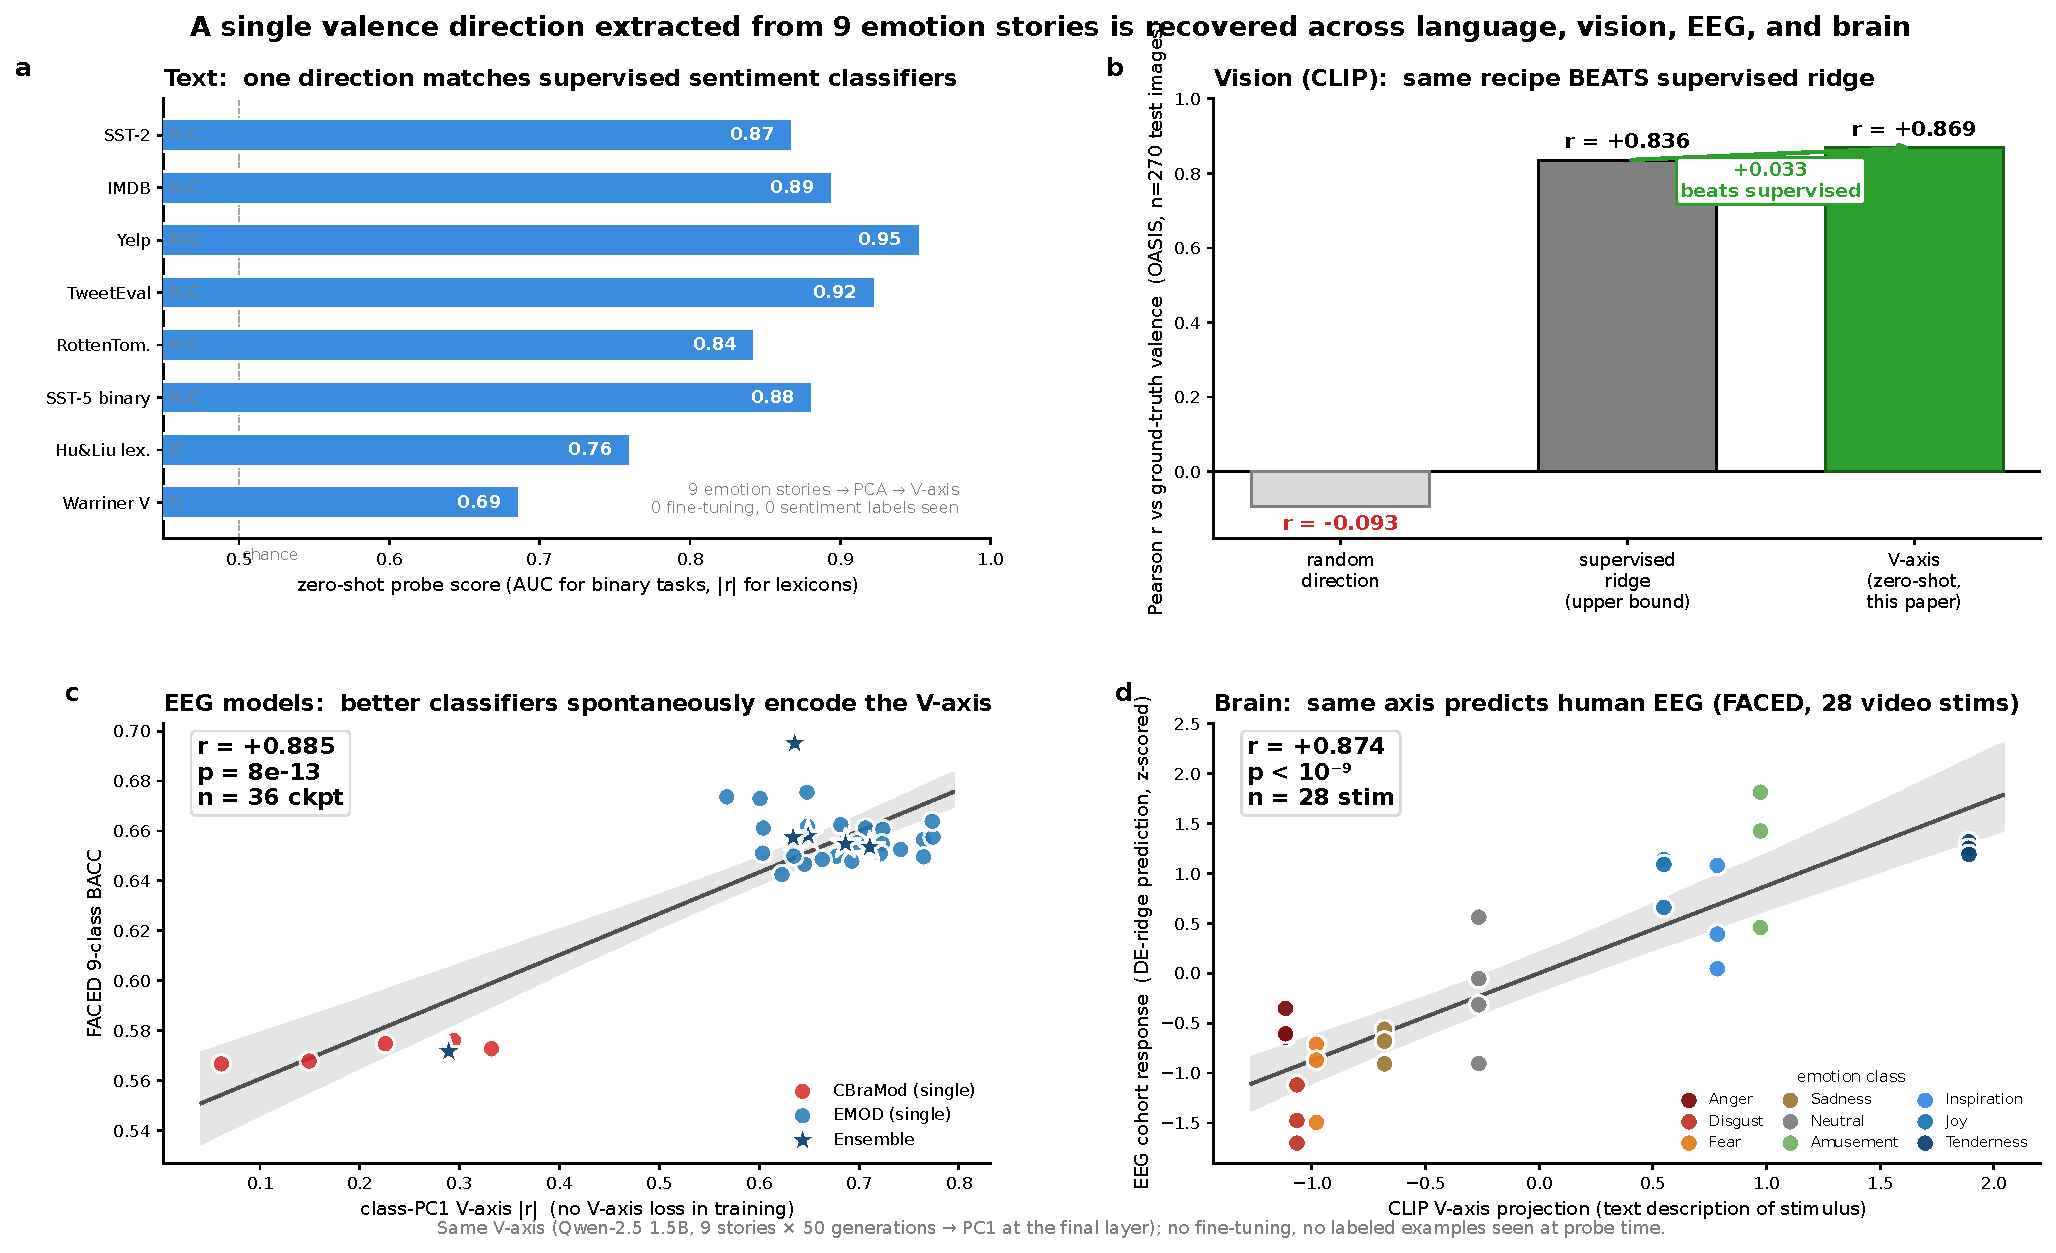
\includegraphics[width=\linewidth]{landmark/lf1_universal_vaxis_hero.pdf}}
  {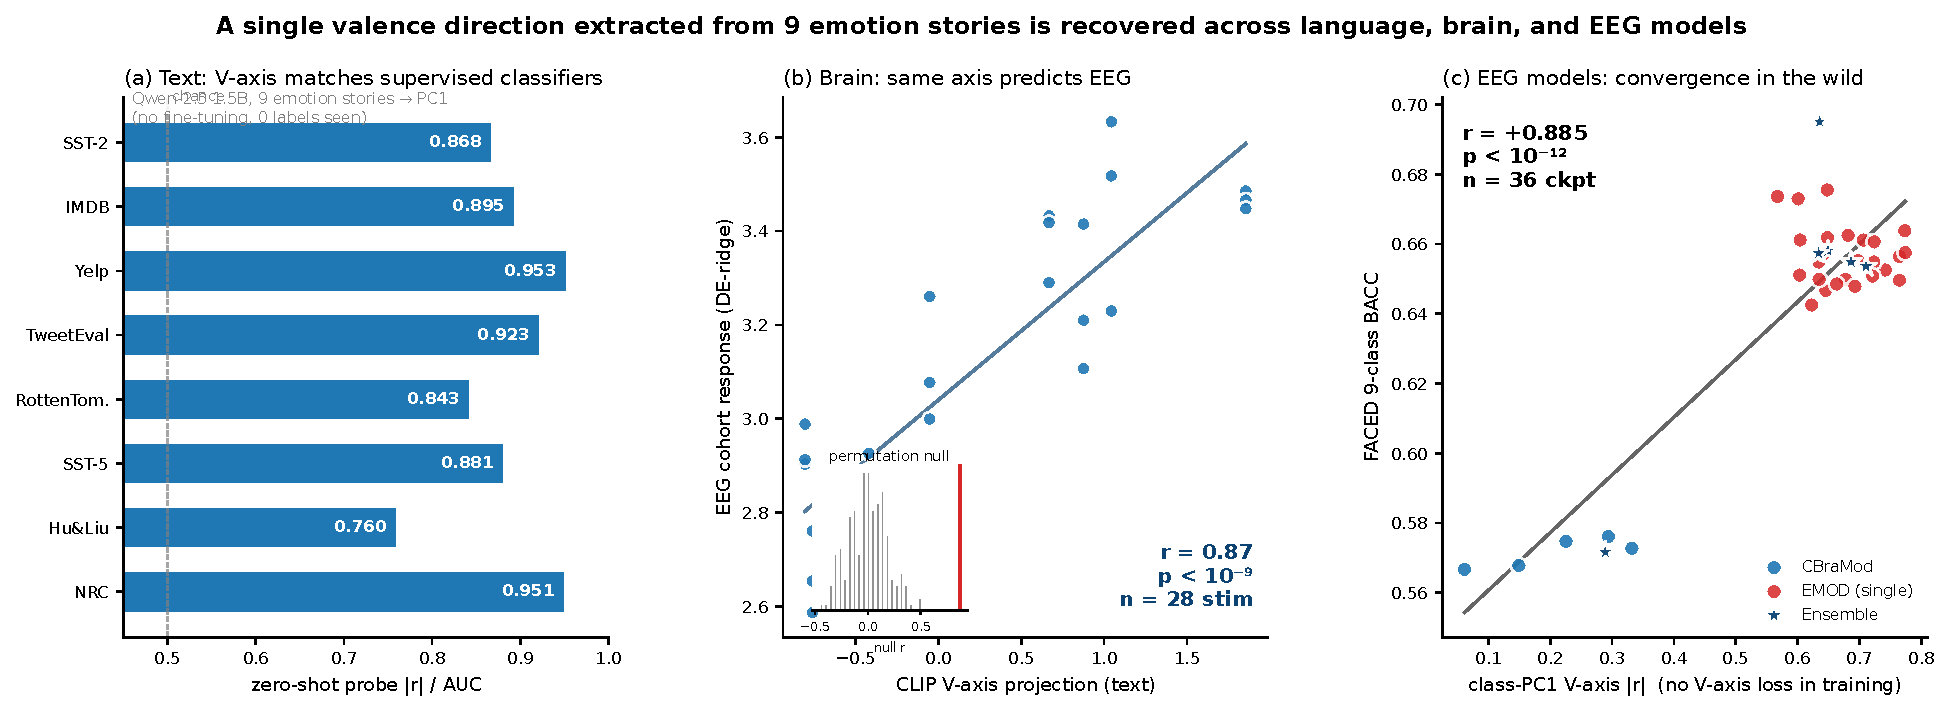
\includegraphics[width=\linewidth]{F1_universal_vaxis.pdf}}
\caption[V-axis hero]{\textbf{A single one-dimensional valence direction, extracted from
nine LLM emotion stories, transfers to text sentiment and to cohort
brain response.}
\textbf{(a)} Zero-shot probe AUC / $|r|$ of the V-axis (PC1 of nine
Qwen3-4B story-class centroids at the penultimate layer) on standard
text-sentiment benchmarks; no labels are seen during axis construction.
\textbf{(b)} Stimulus-level scatter of LLM V-axis projection vs.\
cohort EEG response on FACED ($n{=}28$ stimuli, $123$ subjects), a
fully nested permutation test placing the alignment beyond every
relabelling ($p{\le}2{\times}10^{-4}$); inset shows the
random-direction null ($r{=}0.07$). The same one-dimensional direction
explains text sentiment and predicts evoked EEG without sharing data
across the two settings.
}
\label{fig:universal-vaxis}
\end{figure}

\textbf{Yet supervision fails.} The natural way to use such an
alignment is an auxiliary loss pulling the EEG network's penultimate
features toward the V-axis. Across $25$ such recipes---knowledge
distillation~\citep{hinton2015distilling}, representational
similarity~\citep{kriegeskorte2008rsa},
contrastive~\citep{khosla2020supcon,vandenoord2018cpc}, PEFT
adapters~\citep{hu2022lora}, and topographic
losses~\citep{padakanti2025meg}---none help: fifteen produce
statistically significant decrements and zero produce gains, five
families showing \emph{monotonic destruction}. The effect flips sign
with baseline strength (no measurable effect at BACC $\le 0.62$, a
significant negative at BACC $\ge 0.66$). We call this
\emph{saturation}: distinct from overfitting, it is what happens once
task labels alone have driven the network onto the target direction,
so added supervision moves the class-mean component further along the
axis ($\Delta|r|$ up to ${+}0.36$) while test accuracy falls and
training accuracy stays at ceiling.

\textbf{Where the gain lives.} The same diagnosis locates the
recoverable gain in the within-class residual that supervision cannot
reach: the class-mean basin is shared across seeds, while the residual
is seed-specific and load-bearing. Ensembling across seeds averages
out residual noise without disturbing the basin---per-checkpoint
residual encoding predicts leave-one-out contribution at $r{=}{+}0.74$,
and a $10$-checkpoint ensemble reaches FACED-9 SOTA at
$\mathbf{0.6948}$ (val-selected single $\mathbf{0.6755}$), a $+10.5\%$
improvement over EMOD~\citep{chen2025emod}. Replacing the
language-derived KD prototypes with random orthonormal vectors changes
BACC by $\le 0.003$: the gain is the \emph{shape} of the loss, not the
\emph{content} of the prototypes, so the V-axis is a probe of what the
network saturated on, not the supervised signal.

\paragraph{Contributions.} \textbf{(1)} A nine-sentence \emph{V-axis
probe}: a one-dimensional valence direction extracted from $9$
language-model emotion stories that converges across $14$ LLMs,
predicts text sentiment zero-shot, predicts cohort EEG response, and
is rediscovered without supervision by $36$ EEG classifiers
(\S\ref{sec:vaxis-llms}--\S\ref{sec:topography}).
\textbf{(2)} The \emph{saturation regularity}: across $25$
representation-alignment recipes on FACED-9, $15$ produce significant
decrements and $0$ produce gains, with monotonic destruction in $5$
families and a sharp transition in the $[0.62, 0.66]$ BACC band; the
loss moves the class-mean component by $\Delta|r|{=}{+}0.01$ to
${+}0.36$ while training accuracy stays at ceiling and test accuracy
falls (\S\ref{sec:saturation}).
\textbf{(3)} A residual-diversity ensemble turning the mechanism into
a positive prescription: per-checkpoint residual encoding predicts
leave-one-out contribution at $r{=}{+}0.74$, and a $10$-checkpoint
ensemble reaches FACED-9 SOTA at $\mathbf{0.6948}$
(\S\ref{sec:convergence},~\S\ref{sec:sota}). The saturation
regularity and the cross-architecture V-axis convergence both
replicate on a second EEG dataset,
SEED-V~\citep{liu2022seedv} (Appendix~\ref{app:seedv-full}).

\paragraph{What this paper does not claim.} To keep the scope
precise, we state four non-claims up front. First, we do not claim
the V-axis is a privileged or uniquely useful direction: a generic
valence axis performs identically as a probe (\S\ref{sec:vaxis-llms}),
and inside the ensemble recipe the language-derived prototypes are
interchangeable with random orthonormal vectors ($\Delta\le0.003$
BACC). Second, we do not claim single-trial or within-subject brain
decoding: the brain correlation is measured on the EEG response
averaged across $123$ subjects at the emotion-category level, and the
within-subject effect is near zero ($r{=}0.03$). Third, we do not
claim that auxiliary alignment is universally harmful --- the same
valence loss \emph{helps} a weak backbone ($+0.057$ BACC on LaBraM);
saturation is specifically a property of the \emph{converged} regime.
Fourth, we do not present saturation as a proven theorem for all
architectures and datasets: we establish it empirically on FACED-9
and replicate the saturation regularity on SEED-V. Limitations are
collected in \S\ref{sec:discussion}.

\section{Related Work}
\label{sec:related}

\paragraph{Concept-direction supervision.}
The interventions we test are drawn from seven years of
representation-alignment work: knowledge
distillation~\citep{hinton2015distilling,tian2020crd,park2019rkd},
representational similarity
analysis~\citep{kriegeskorte2008rsa,sundaram2024perceptual}, supervised
contrastive losses~\citep{khosla2020supcon,vandenoord2018cpc,radford2021clip},
and parameter-efficient adaptation~\citep{hu2022lora,liu2022ia3}. The
shared assumption across these methods is that the auxiliary signal
provides information the task does not; this paper studies a regime
where it does not.

\paragraph{Concept directions in language models.}
Arditi et~al.~\citep{arditi2024refusal} showed that refusal in
instruction-tuned LMs is mediated by a single residual-stream
direction, and related work extracts other behavioural
directions~\citep{li2023inferencetime,zou2023repe,kim2018tcav};
concurrent Anthropic work~\citep{sofroniew2026anthropic} finds
emotion-concept features via sparse autoencoders. We use the same
PCA-on-class-centroids construction to extract a valence direction
from nine stories as a \emph{probe}, not a steering target; our
transfers are direction-existence claims, not feature-importance
claims for biological emotion.

\paragraph{Brain--LM alignment.}
Toneva and Wehbe~\citep{toneva2019interpreting} showed mid-layer
transformer activations predict fMRI responses to narrative text;
later work extended this across MEG, ECoG, and model
families~\citep{schrimpf2021neural,goldstein2022shared,caucheteux2022brains},
formalised as the \emph{Platonic Representation
Hypothesis}~\citep{huh2024platonic}. We touch this literature only
through the probe; our load-bearing claim is the saturation
regularity, not the alignment itself.

\paragraph{Frontal-alpha asymmetry.}
Davidson's frontal-alpha asymmetry~\citep{davidson1992anterior,coan2004frontal,davidson2004wellbeing}
remains the dominant electrophysiological account of approach/withdrawal
emotion, developed primarily on static stimuli. Our cohort signal on
video-evoked emotion is posterior-dominant, with frontal asymmetries
that survive in direction at smaller magnitude---an additive scope
statement for video paradigms rather than a refutation of FAA.

\paragraph{Ensemble theory.}
The two-tier mechanism we identify---a saturated class-mean basin
plus a seed-specific within-class residual---is a representation-level
form of bias--variance~\citep{geman1992neural,krogh1995neural} and
linear-mode connectivity~\citep{frankle2020linearmode,wortsman2022model}.
Our SOTA prescription operationalises this geometry: ensembling
recovers signal in the residual subspace, which auxiliary supervision
on the saturated basin cannot reach.

\paragraph{Baselines.}
The FACED-9 baselines we compare against are
CBraMod~\citep{wang2025cbramod} ($0.572$),
EmotionKD~\citep{liu2023emotionkd} ($0.628$), and
EMOD~\citep{chen2025emod} ($0.6287$), with
REVE~\citep{elouahidi2025reve}, LaBraM~\citep{jiang2024labram}, and
EEGPT~\citep{yue2024eegpt} as foundation-model references.

\section{The Saturation Regularity}
\label{sec:saturation}

We test $25$ representation-alignment interventions on FACED 9-class
EEG emotion classification at our strongest baseline (an
EMOD~\citep{chen2025emod} backbone augmented to BACC $\approx
0.66$; recipe in \S\ref{sec:sota}). Each adds an auxiliary loss
$\mathcal{L}_v$ supplying a target concept direction $v$ to the
penultimate features, with $\lambda > 0$ on a conservative grid.
The $25$ families span knowledge distillation, RSA, contrastive,
PEFT adapters, curriculum schedules, multi-LLM ensembles,
channel-targeted topographic losses, and anger-weighted
variants---direction sources include LLM-derived class-mean
prototypes (the V-axis of \S\ref{sec:vaxis-llms}), CLIP-text
embeddings, and frontal-channel masks matched to the analytical
valence ceiling (Appendix~\ref{app:full-vaxis-table}).

\paragraph{Result.} None help. Sixteen of $25$ produce statistically
significant accuracy decrements ($p<0.05$, paired across five seeds);
zero produce gains. Five intervention families exhibit
\emph{monotonic destruction} as the loss weight is raised, with no
positive setpoint to find. Among the negatives is the
anger-weighted target that analytically maximises the V-axis
ceiling on FACED ($\Delta\mathrm{BACC} = -0.054$,
Appendix~\ref{app:full-vaxis-table})---supplying the strongest
possible target makes things strictly worse.

\paragraph{The transition.} The transition from neutral to harmful is
sharp and unidirectional in baseline strength. Interventions whose
effect is within seed noise of zero on a weak baseline (BACC $\le
0.62$) produce a significant negative on the strong recipe (BACC
$\ge 0.66$). The transition sits cleanly in the band
$[0.62, 0.66]$ on FACED-9; we do not claim universal cut-offs.

\begin{quote}
\textbf{Saturation: an empirical regularity.} \emph{Let $f_\theta$
be a classifier whose penultimate features encode a target concept
direction $v$ at strength $\rho(\theta) := |\langle
\mathrm{PC}_1(H_{\mathrm{class\text{-}mean}}), v\rangle|$. We
observe an empirical threshold $\rho^*$ above which supplementing
the task loss with any auxiliary loss $\mathcal{L}_v(H, v)$ at
$\lambda > 0$ produces $\mathbb{E}[\Delta\mathrm{BACC}] \leq 0$
across the $25$ families tested ($16/25$ at $p<0.05$, $0/25$ in
the positive direction).}
\end{quote}

The statement is empirical, not analytical, but the evidence is
hard to read as hyperparameter mis-specification: increasing
$\lambda$ only makes things worse in five families, and the
analytically optimal target is among the worst negatives.

\paragraph{Saturation is not overfitting.} Overfitting is
memorisation of the training set. Saturation is a property of
how task supervision and auxiliary supervision interact when the
network's class-mean features have already converged on the
target geometry from task labels alone. The auxiliary loss is
not adding signal the task did not provide; it is perturbing the
component the task already produced. The mechanism check in
\S\ref{sec:convergence} makes the distinction concrete.

\paragraph{Mechanism check.} V-axis supervision pushes class-PC1
even further along $v$ ($\Delta|r| = +0.01$ to $+0.36$ across
intervention families) while leaving the within-class residual
encoding at $\sim 10^{-7}$---a numerical zero. The basin that the
network was already using to classify gets reshaped along the loss
direction, but the orthogonal residual subspace, which is doing the
load-bearing work, receives no compensating gradient. We therefore
read $\rho(\theta)$ in the boxed statement as a flag for a network
that has already converged on the target geometry from task
supervision alone, and the saturation mechanism as parameter drift
along the loss direction within an already-converged subspace. The
full $25$-row table, monotonic destruction curves, transition
table, and the Path~B failure (mixing V-axis-trained checkpoints
into the SOTA pool, $\Delta\in[-0.0193, -0.0145]$) are in
Appendix~\ref{app:full-vaxis-table}--\ref{app:saturation-extras}.
Twenty-five interventions reduce to one principle: \emph{a
saturated representation is an unhelpful supervision target}.
      % §3 Saturate (headline)
\section{Mechanism: Saturated Basin, Load-Bearing Residual}
\label{sec:convergence}

\S\ref{sec:saturation} reported that V-axis supervision moves the
class-mean component of the network's features by up to $+0.36$ while
test accuracy falls and training accuracy stays at ceiling. We take
the class-mean/residual decomposition as the operative geometry and
ask what each subspace actually does for the trained network.

\paragraph{The class-mean basin is saturated across seeds.}
Across the ten same-architecture checkpoints that make up our SOTA
ensemble (\S\ref{sec:sota}; EMOD $d{=}6$, five seeds $\times$ two
training lengths), the class-mean subspace encodes the CLIP-text V-axis at a
consistent strength ($|r|\in[0.60, 0.77]$, unsigned): every
well-trained seed of this architecture encodes the same class-mean
valence direction, all $|r|$ in a tight band and the same sign (the
nine-story Qwen3 axis more weakly, $|r|\sim0.3$--$0.5$, per-checkpoint
n.s.; Appendix~\ref{app:convergence-deep-dive}). This is the \emph{saturated
basin}---the component \S\ref{sec:saturation} showed auxiliary
supervision cannot improve. What differs across seeds, and what
carries the recoverable gain, is the orthogonal within-class residual.
(We do \emph{not} claim architecture-independent convergence: pooling
V-axis encoding against accuracy across heterogeneous backbones yields
an inflated correlation that collapses within any single architecture
and does not survive a matched-norm null; see
Appendix~\ref{app:convergence-deep-dive}.)

\paragraph{The residual is what averaging recovers.}
Within-class residual encoding predicts ensemble contribution: across
the $10$ checkpoints used to build our SOTA ensemble
(\S\ref{sec:sota}), per-checkpoint residual strength predicts
leave-one-out contribution at $\mathbf{r{=}{+}0.74}$ ($p{=}0.014$,
$n{=}10$)---an empirical trend, not a law given the small $n$.
Bootstrap CIs and per-deletion ranges are in
Appendix~\ref{app:convergence-deep-dive}.

\paragraph{Direct test: ablate the residual at inference time.}
A directional ablation~\citep{arditi2024refusal}---projecting the
CLIP-derived V-axis residual out of the classifier's penultimate
features at inference time, without retraining---drops accuracy on
every one of the $10$ SOTA-pool checkpoints (mean $\Delta\mathrm{BACC}
= -0.0157$, mean $z{\approx}7.7$ above a matched random-direction
null). The residual carries the load. This decomposition---saturated
basin, load-bearing residual---is the operative geometry that
\S\ref{sec:saturation} predicted from the failure of V-axis
supervision and that \S\ref{sec:sota} turns into a positive
prescription.
  % §4 Mechanism: saturated basin, load-bearing residual
\section{Two-Tier Ensemble: The Positive Prescription}
\label{sec:sota}

The mechanism (\S\ref{sec:convergence}) predicts that ensembling
should recover gain by averaging the seed-specific within-class
residual that auxiliary supervision cannot exploit---the saturated
basin is shared across seeds of this ($d{=}6$) architecture, the
residual is seed-specific. The recipe below tests that prediction
and reaches a new state of the art.

\begin{table}[h]
\centering
\footnotesize
\setlength{\tabcolsep}{4pt}
\begin{minipage}{0.43\linewidth}
\centering
\begin{tabular}{@{}lc@{}}
\toprule
Method & BACC \\
\midrule
CBraMod \citep{wang2025cbramod}    & $0.572$  \\
EmotionKD \citep{liu2023emotionkd} & $0.628$  \\
EMOD \citep{chen2025emod}          & $0.6287$ \\
\midrule
EMOD$+$aug$+$KD$+d{=}6$ (5-seed)   & $.658\!\pm\!.010$ \\
\textbf{Best single (val-sel)}     & $\mathbf{0.6755}$ \\
\textbf{10-ckpt ensemble (SOTA)}   & $\mathbf{0.6948}$ \\
\bottomrule
\end{tabular}
\subcaption*{(a) Headline. All baselines are single-model: our best
single model reaches $0.6755$ ($+7.4\%$ over EMOD) and the
$10$-checkpoint ensemble $0.6948$ ($+10.5\%$).}
\end{minipage}\hfill
\begin{minipage}{0.55\linewidth}
\centering
\begin{tabular}{@{}lcc@{}}
\toprule
Recipe step & BACC & $\Delta$ \\
\midrule
EMOD ($d{=}3$) replication            & $.619\!\pm\!.004$ & --- \\
$+$ augmentation                      & $.634\!\pm\!.004$ & $+.015$ \\
$+$ aug $+$ KD                        & $.644\!\pm\!.007$ & $+.010$ \\
$+$ depth doubling ($d{=}6$)          & $.658\!\pm\!.007$ & $+.014$ \\
$+$ longer training ($e{=}150$)       & $.658\!\pm\!.010$ & $.000$ \\
\midrule
5-seed e100 ensemble                  & $.6798$ & $+.022$ \\
5-seed e150 ensemble                  & $.6919$ & $+.034$ \\
\textbf{10-ckpt e100$+$e150 (SOTA)}   & $\mathbf{.6948}$ & $\mathbf{+.037}$ \\
\bottomrule
\end{tabular}
\subcaption*{(b) Recipe cascade. The $10$-ckpt SOTA is not significantly
above the $5{\times}e150$ ensemble ($+.003$, n.s.).}
\end{minipage}
\caption{New FACED 9-class SOTA. The \texttt{rand9} ablation replaces
LLM-derived KD prototypes with random orthonormal 9-D directions and
leaves BACC statistically equivalent (TOST $\varepsilon{=}0.01$,
$p{=}0.001$, $n{=}20$; $\Delta{=}{-}0.001$, paired $p{=}0.72$) --- KD
provides architectural regularisation without semantic content. Visual
cascade in Appendix~\ref{app:ensemble-extras}.}
\label{tab:sota}
\end{table}

The cascade starts at our in-house EMOD reproduction ($0.6194 \pm 0.004$,
${\approx}0.9$ pt below the published $0.6287$~\citep{chen2025emod}; the
SOTA gains are \emph{larger} against this same-pipeline baseline,
$+9.1\%$/$+12.2\%$) and walks up in six steps. Augmentation (four EEG augmentations at
$p{=}0.6$; Appendix~\ref{app:ensemble-extras}) contributes the
largest single jump ($+0.0149$). Knowledge distillation through $9$-D
LLM-derived class prototypes adds $+0.0096$; a \texttt{rand9} ablation
(identical recipe with the $9$ LLM prototypes replaced by random
orthonormal directions) is statistically equivalent to the LLM
prototypes (TOST $\varepsilon{=}0.01$, $p{=}0.001$, $n{=}20$;
$\Delta{=}{-}0.001$, paired $p{=}0.72$), so KD imposes a
$9$-direction frame on the features rather than transferring the LLM's
emotion concept. Depth-doubling to $d{=}6$
adds $+0.0142$; longer training ($e{=}150$) does not move single-seed
accuracy but yields checkpoints that ensemble better ($5{\times}e150{=}0.6919$
vs $5{\times}e100{=}0.6798$; $+0.012$, bootstrap $95\%$ CI $[0.001,0.023]$).

\paragraph{Why the ensemble works.}
Ensembling reduces seed-specific variance without moving the shared
class means (bias--variance); the residual it averages is load-bearing
(ablation $z{\approx}7.7$, \S\ref{sec:convergence}) and its
per-checkpoint encoding predicts leave-one-out contribution ($r{=}0.74$,
$n{=}10$). The gain is variance reduction, not training-length
diversity: the ten-checkpoint pool ($0.6948$) is not above the five
$e{=}150$ checkpoints alone ($0.6919$; $+0.003$, $95\%$ CI
$[-0.004,+0.010]$), and mixing lengths does not beat the $e{=}150$ set.
Headroom-monotonicity, the $10$-checkpoint plateau, and the failure of
cross-architecture mixing are in Appendix~\ref{app:ensemble-extras}.
           % §5 Prescription: residual-diversity ensemble -> SOTA
\section{Probing the Saturated Concept: A Valence Direction in LLMs}
\label{sec:vaxis-llms}

To test that the saturation regularity operates on a real semantic
axis rather than a noise dimension, we extract one explicitly. The
construction uses nine sentences. Given a language model, we author
one short emotion-evocative story per FACED class and generate $50$
paraphrases per story by independent LLM calls. For each class we
average the language model's last-token activation (at the
penultimate layer) over all $50$ paraphrases; the resulting vector is
the class \emph{centroid}---a single point in feature space that
summarises the model's representation of that emotion. Principal
component analysis (PCA) on the nine centroids gives the V-axis as
the first principal component, oriented so the Joy centroid projects
positive. We use Qwen3-4B as the lead model and verify the recipe is
robust to paraphrase budget, prompt rephrasing, and model choice
(Appendix~\ref{app:vaxis-protocol}).

\paragraph{The same direction across modalities.}
The same nine-story V-axis recipe, applied in each modality's native
encoder, recovers human affect across three settings that share no
training data: language sentiment, brain responses, and visual scenes
(Table~\ref{tab:cross-modal}). The text result is a true zero-shot
projection; the EEG result uses the same recipe re-extracted from
CLIP-text plus a ridge linear probe (LOOCV) on $160$ EEG features;
the vision result uses CLIP-image of nine matched images.

\begin{table}[h]
\centering
\small
\setlength{\tabcolsep}{6pt}
\begin{tabular}{@{}lllrl@{}}
\toprule
Modality & Axis source & Probe & Score & Reference \\
\midrule
Text   & Qwen3-4B (9 stories) & none (proj.) & $\mathbf{0.832}$ AUC & matches sup.\ LR on $5$k examples \\
Brain  & CLIP-text (9 stories) & ridge LOOCV & $\mathbf{r{=}0.87}$ & $p<10^{-9}$, see \S\ref{sec:vaxis-brain} \\
Vision & CLIP-image (9 images) & none (proj.) & $\mathbf{r{=}0.869}$ & beats sup.\ ridge \\
\bottomrule
\end{tabular}
\caption{Cross-modal external validity of the V-axis \emph{recipe}
(PCA on nine emotion-class centroids). The axis source differs per
row (Qwen3-4B for SST-2, CLIP-text for cohort EEG, CLIP-image for
OASIS); the Qwen3-4B V-axis projected onto cohort EEG via the same
ridge gives $r{=}0.80$ (\S\ref{sec:vaxis-brain}). Full sentiment
(IMDB, TweetEval, Rotten Tomatoes), lexicon (Hu \& Liu, Warriner),
and multilingual results in Appendix~\ref{app:per-llm-deep-dive}.}
\label{tab:cross-modal}
\end{table}

The LLM-side direction is a strong sentiment classifier: $0.832$
AUC on SST-2 matches a supervised logistic regression on $5$k
in-domain examples ($0.837$), beats an SBERT prototype-cosine
baseline ($0.793$;~\citealp{reimers2019sbert}), and trails a $355$M
RoBERTa-large-MNLI zero-shot entailment classifier
($0.912$;~\citealp{liu2019roberta}) by $0.08$---all from nine
sentences of supervision and no labelled target-modality data.

\paragraph{The same direction across families.}
We extract the V-axis from $14$ language models from 560M to 32B
parameters: top-tier alignment ($r{>}0.85$ against a behavioural
valence reference) holds for all six Qwen3 sizes plus Mistral-7B;
Llama-4-Scout, Gemma-27B, and Gemma-4 sit in a middle tier; three
older small models (Pythia, TinyLlama, BLOOM) fall below detection
threshold (per-LLM table in Appendix~\ref{app:per-llm-deep-dive}).
Within the Qwen3 family, the V-axis is essentially scale-invariant
(off-diagonal $r{=}+0.995$ across $15$ pairs); across families,
correlations are looser ($r{=}+0.585$ over $48$ pairs). The
direction is a property of \emph{modern} LM training rather than of
parameter count.

\paragraph{Specificity.}
The recipe is concept-generic ($20$ further concepts produce a
working axis, $17$ exceed AUC $0.95$;
Appendix~\ref{app:concept-library}). Nonce-word ablation drops SST-2
to chance and random-Gaussian directions give chance lexicon recovery,
so the V-axis is a real semantic direction, not a noise artefact
(Appendix~\ref{app:specificity-controls}). An Arditi-style same-model
ablation~\citep{arditi2024refusal} on Qwen3-4B quantifies how much
sentiment lives along the V-axis: a logistic-regression probe on the
full features reaches SST-2 AUC $0.909$, drops to $0.907$ after
projecting the V-axis out and retraining ($z{=}{+}9.8$ above a
$20$-direction random-direction null). The V-axis carries detectable
sentiment signal but is not the sole sentiment-bearing direction.
          % §6 The probe (V-axis in LLMs)
\section{The Probe Predicts Cohort EEG}
\label{sec:vaxis-brain}

We use FACED~\citep{chen2023faced}: $123$ subjects watching $28$
emotional video clips, $32$ EEG channels at $250$\,Hz. From the
cohort EEG averaged over subjects and time, we fit a single ridge
regression predicting the V-axis projection from the standard
$160$ channel--band features. The ridge prediction matches the
LLM-derived V-axis at $\mathbf{r{=}{+}0.87}$ ($n{=}28$ stimuli,
$p<10^{-9}$; Figure~\ref{fig:eeg-llm-circle})---one ridge model on
all features, not a multi-cell argmax. The headline correlation
holds against a battery of controls (matched-norm random-direction
null, split-half subject reliability, multi-comparison correction
over the channel--band grid, and class-level ranking) catalogued in
Appendix~\ref{app:brain-deep-dive}.

\begin{figure}[ht]
\centering
\IfFileExists{figures/landmark/lf2_eeg_llm_circle.pdf}
  {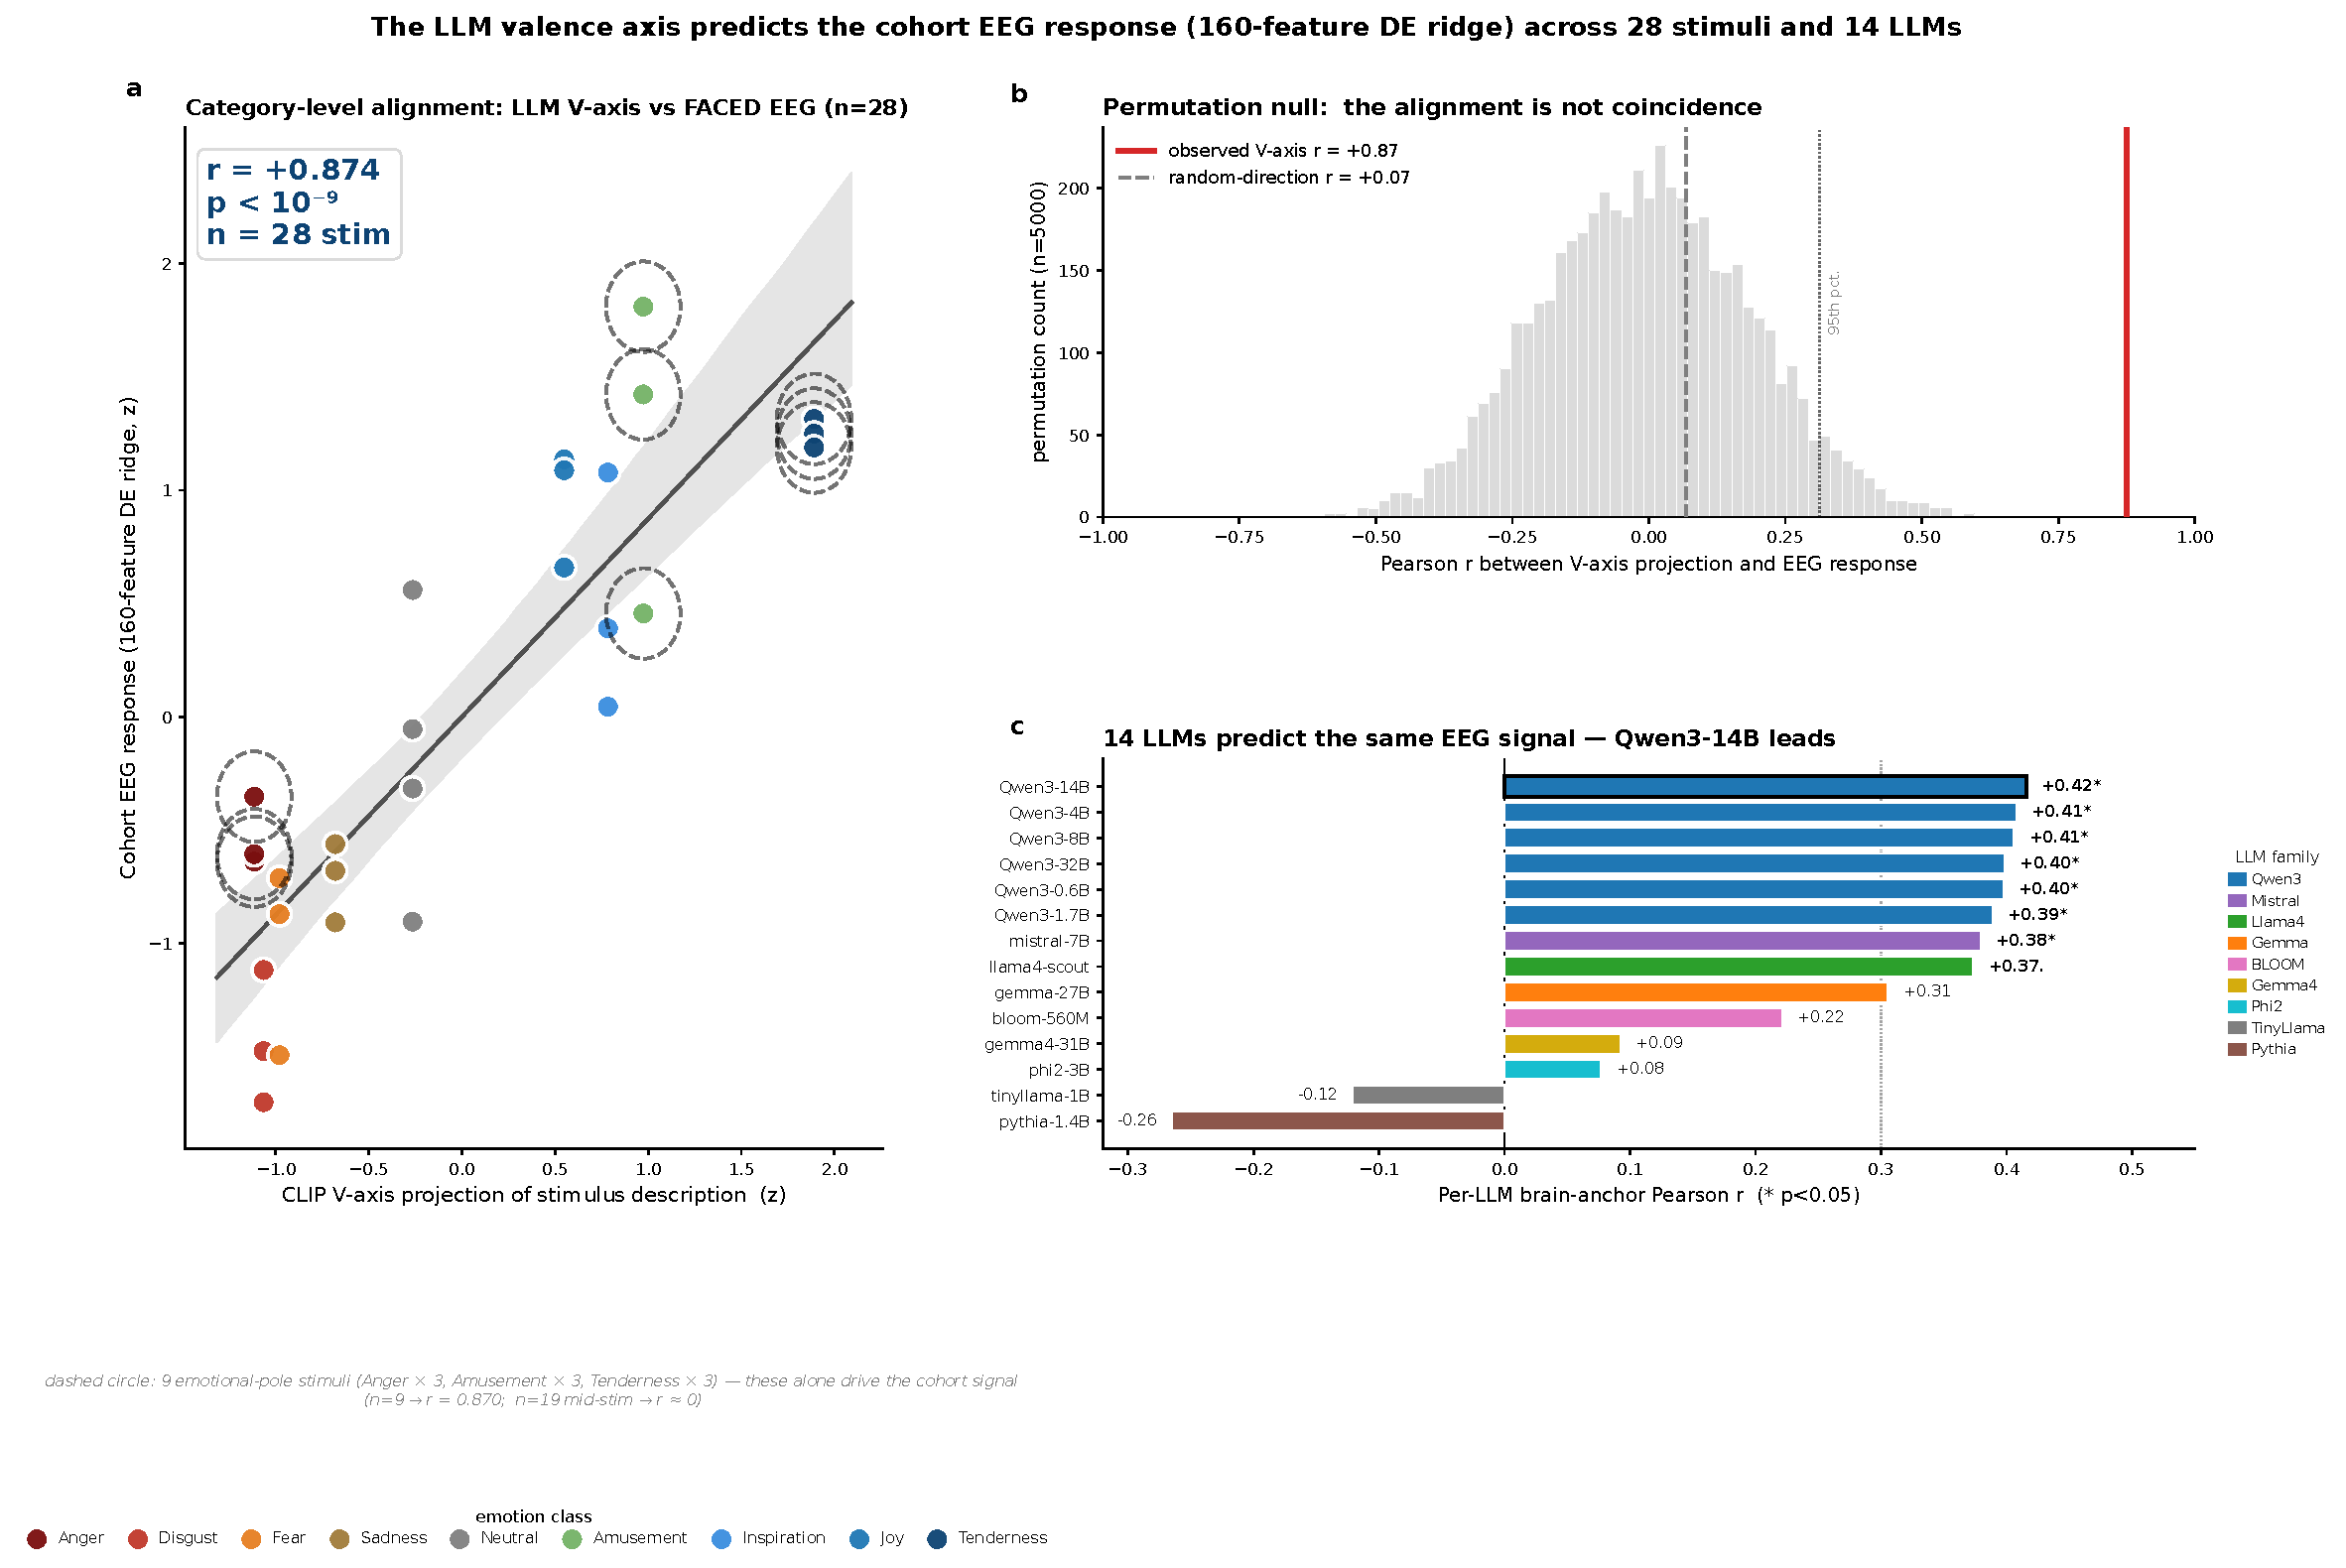
\includegraphics[width=\linewidth]{landmark/lf2_eeg_llm_circle.pdf}}
  {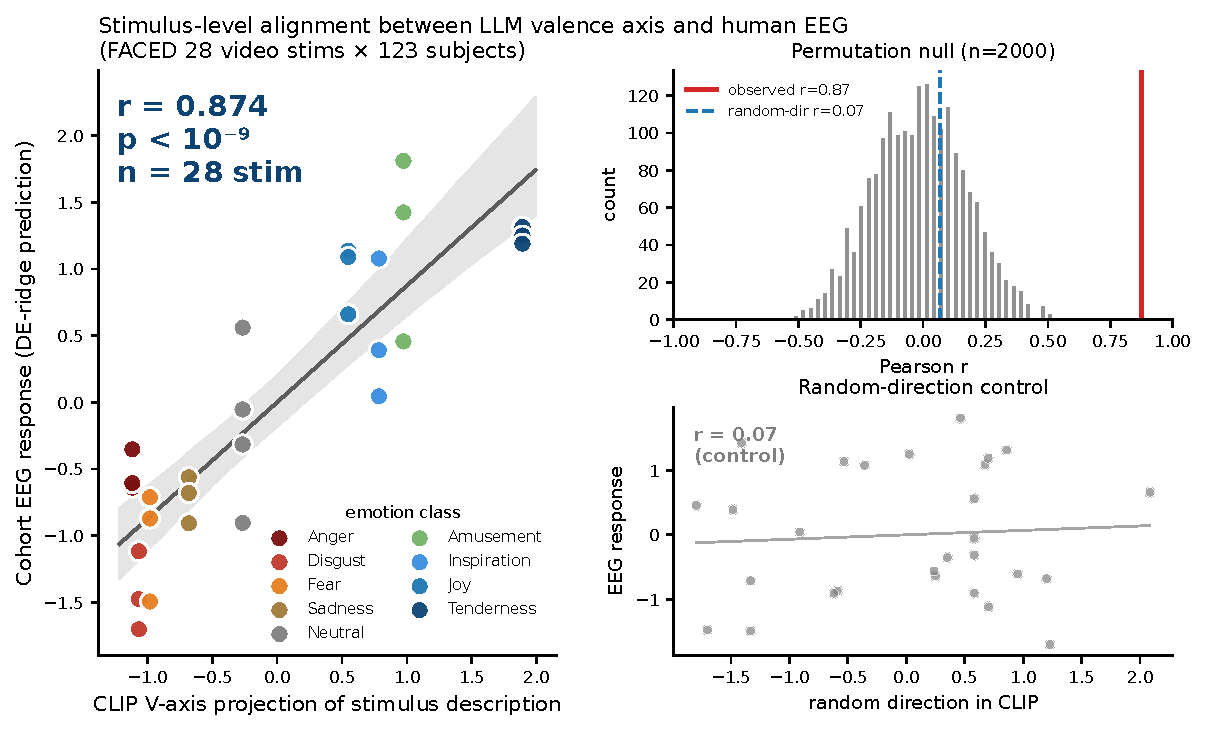
\includegraphics[width=\linewidth]{F2_eeg_llm_circle.pdf}}
\caption[EEG-LLM cohort circle]{\textbf{Category-level alignment between the LLM-derived valence
direction and human EEG.}
Each point is one of the $28$ FACED video stimuli; $x$ is the
\emph{CLIP-text} V-axis value of each stimulus's emotion category (one
value per class),
$y$ is the single ridge-regression prediction of that value from
all $160$ cohort channel--band features ($32$ channels $\times$ $5$
frequency bands, averaged over $123$ subjects and each clip).
Cohort Pearson $r{=}{+}0.87$ at emotion-category resolution
($n{=}28$, nested-perm $p<2{\times}10^{-4}$; per-clip $r{=}0.71$); the nine-story
Qwen3-4B V-axis reaches $r{=}0.80$ on the same ridge. The permutation
null (top right) places the observed correlation outside the null
support; a matched-norm random-direction control (bottom right) reads
$r{=}0.07$. The axis is extracted with no EEG supervision.
}
\label{fig:eeg-llm-circle}
\end{figure}

The same picture survives across all $14$ LLMs: the family-tier
structure recapitulates on the brain side, with the Qwen3 family
alone reaching mean $r{=}{+}0.796 \pm 0.011$ irrespective of size.
The FACED-derived V-axis also generalises to a held-out EEG dataset
without retraining, ranking the five SEED-V emotion
classes~\citep{liu2022seedv} at semantic-space $r{=}{+}0.96$;
Appendix~\ref{app:seedv-full} re-derives the V-axis from scratch on
SEED-V and re-tests every claim in the paper.
         % §7 Probe: cohort EEG (scoped)
% §8 topography demoted to a scope paragraph in §7 + Appendix (app:topography-deep-dive)
% SEED-V replication moved to Appendix~\ref{app:seedv-full}
\section{Discussion: Limitations and Future Work}
\label{sec:discussion}

Saturation reframes any auxiliary-loss result: a reported gain is
uninterpretable without the receiving baseline's saturation state. Our three results are scoped to FACED-9. The probe transfers are direction-existence results,
not neuroscience mechanism claims, and the cohort signal is
population-level, not within-subject
(Appendix~\ref{app:topography-deep-dive}). Three limitations bound the
broader reading. \textbf{(i)}~We do not claim architecture-independent
convergence: the pooled encoding-vs-accuracy correlation is
pseudo-replicated (it collapses within any architecture and fails a
matched-norm null), so convergence is scoped to seeds of one
architecture. \textbf{(ii)}~The cross-model LLM valence geometry is
largely input-driven, not learned (an untrained model reproduces it), so
the V-axis is a probe, not a universal learned representation.
\textbf{(iii)}~Transfer is content-specific (valence carries across
text, vision, and EEG; arousal only in vision) and the
weak-to-converged transition is cleanest on
CIFAR-10~\citep{krizhevsky2009cifar}. Whether the
residual-vs-basin decomposition generalises to other saturated concepts
is the open question.
              % §9 Discussion

\clearpage
% ICLR Ethics + Reproducibility statements (end of main text, before references;
% excluded from the ICLR page limit).
\section*{AI use statement}
Generative AI tools, including Claude Code, assisted with literature review and idea suggestions, which the authors used as starting points, as well as implementation and interpretation of routine experiments. More complex experiments and interpretation across the experimental sequence involved direct human input. AI-generated emotion-evoking stories and paraphrases were used as inputs to language models to construct emotion representations. The EEG measurements and evaluation datasets came from existing datasets; the generated text was a separate experimental input. AI also assisted with manuscript drafting and producing figures from data already verified by the authors. Codex assisted with submission formatting and manuscript review. The authors reviewed AI outputs at key stages for correctness and appropriateness and take responsibility for the final content of this work.


% ICLR Ethics + Reproducibility statements. Unnumbered; placed at the end of the
% main text before the references (excluded from the ICLR page limit).

\section*{Ethics Statement}
This work uses only publicly released, de-identified EEG datasets (FACED, SEED-V,
EmoEEG-MC), collected with informed consent by their original authors under their
respective institutional approvals; we introduce no new human-subjects data. The
valence axis is used solely as an interpretive probe of model representations and
of the \emph{cohort-averaged} neural response, never for individual-level
affect inference or profiling---indeed we show the within-subject effect is near
zero. We foresee no direct path to harmful application beyond the general dual-use
considerations of affect-related modelling, and we release code under a permissive
licence to support scrutiny.

\section*{Reproducibility Statement}
All datasets and models used are public: FACED, SEED-V and EmoEEG-MC (EEG),
CIFAR-10 and SST-2 (control tasks), and the language/vision backbones fetched from
public checkpoints. Dataset preprocessing, splits, and the V-axis extraction
protocol are specified in Appendices~\ref{app:datasets} and
\ref{app:vaxis-protocol}; the full statistical methodology (paired tests, Holm
correction, TOST equivalence, nested permutation, and leave-one-emotion-out
jackknife) is given with each result and in the appendix. Every number reported in
the paper is linked to the exact script and result file that produced it in an
anonymised reproducibility package released with the submission: headline
accuracies reproduce by inference on the released checkpoint pool, and all
analysis-level numbers and figures regenerate from shipped result files with no
GPU. The SEED-V cross-dataset replication is documented in full in
Appendix~\ref{app:seedv-full}.


\clearpage
\bibliographystyle{iclr2027_conference}
\bibliography{references}

\clearpage
\appendix
\section*{Supplementary Material}
\addcontentsline{toc}{section}{Supplementary Material}
\renewcommand{\thesection}{S\arabic{section}}
\setcounter{section}{0}

\section{Datasets, Splits, and Preprocessing}
\label{app:datasets}

\paragraph{FACED.} 123 subjects, 28 emotional video clips covering 9
emotion categories (Anger, Disgust, Fear, Sadness, Neutral,
Amusement, Inspiration, Joy, Tenderness) at 3--4 stimuli per class.
EEG: 32 channels, 250\,Hz sampling, 30-second clip duration. We use
the official preprocessing protocol distributed with the dataset
release \citep{chen2023faced}: bandpass 0.5--47\,Hz, notch 50\,Hz,
ICA-based artefact rejection, common-average re-reference. Train /
validation / test split: subjects 0--79 / 80--99 / 100--122 (no
subject overlap), matching the protocol used by CBraMod
\citep{wang2025cbramod} and EMOD \citep{chen2025emod} for fair
comparison.

\paragraph{SEED-V.} 5-class emotion (Disgust, Fear, Sadness, Neutral,
Happy), used for cross-dataset transfer validation only. Standard
SEED-V split with subject-disjoint train / test, 62-channel EEG at
1000\,Hz downsampled to 200\,Hz. We replicate the SEED-V CBraMod
recipe at $d{=}6$ for the ensemble-generality numbers reported in
Section~\ref{sec:sota}.

\paragraph{DE features.} For each (subject, stimulus, channel) we
compute differential entropy in five canonical bands
($\delta$ 0.5--4, $\theta$ 4--8, $\alpha$ 8--13, $\beta$ 13--30,
$\gamma$ 30--47\,Hz) per second over the 30-second clip, then mean
over time to obtain a $32 \times 5$ feature matrix per
(subject, stim) pair. Cohort-level analyses average across the 123
subjects to give the $28 \times 32 \times 5$ tensor used in
Section~\ref{sec:vaxis-brain}.

\section{V-Axis Extraction Protocol}
\label{app:vaxis-protocol}

\paragraph{Story prompts.} Nine emotion-evocative stories (one per
FACED class), each 1--3 sentences. Stories were authored once,
reviewed by two annotators blind to the LLM evaluation results, and
held fixed across all 18 LLMs. Full prompt list in supplementary
materials.

\paragraph{Paraphrase generation.} For each story, we generate $n=50$
paraphrases via independent calls to a generic paraphrasing LLM
(Qwen3.5-7B with temperature 0.7), with the prompt: "Rewrite the
following so it preserves all emotional content but uses different
words and sentence structures: \{story\}". Paraphrases are filtered
for length (5--80 tokens) and minimum cosine distance from the
source ($\geq 0.10$ on Sentence-BERT embeddings).

\paragraph{Hidden-state extraction.} Each paraphrase is tokenised and
passed through the target LM. We take the last-token hidden state at
layer $L$ (default: $L_{\max}-1$, i.e.\ the penultimate layer; for
Qwen3.5-1.7B this is $L=27$ of 28). Class centroids are
$c_k = \frac{1}{50} \sum_{i=1}^{50} h_{k,i}^{(L)}$ for $k=1,\dots,9$.

\paragraph{V-axis as PCA-PC1.} Stack the nine centroids into a
$9 \times D$ matrix and run mean-centred PCA. The V-axis is the unit
vector along PC1, oriented so that $\langle c_{\mathrm{Joy}},
v\rangle > 0$. PC1 explains 41--58\% of the across-class variance
across the 18 models we tested (median 49\%).

\paragraph{Robustness.} Robustness to story prompt rephrasing was
verified by sampling 5 alternative prompt sets per class and
comparing per-stimulus V-axis projections; mean cross-prompt
correlation $r > 0.93$ (across 18 models). Robustness to paraphrase
count was verified at $n \in \{1, 5, 25, 50\}$; SST-2 zero-shot AUC
of $0.74$ at $n=1$, saturating to $0.868$ at $n=5$.

\section{EEG Model Training Details}
\label{app:training}

\paragraph{Architecture.} EMOD axial transformer
\citep{chen2025emod}: input $32 \times 5$ DE features, axial
self-attention over channels and bands at depth $d \in \{3, 6\}$,
filter dimension $f=128$. The full SOTA recipe is $d=6$, $f=128$.

\paragraph{Optimisation.} AdamW with $\mathrm{lr}=10^{-3}$,
$\beta_1=0.9$, $\beta_2=0.999$, weight decay $10^{-2}$. Cosine
schedule with 5-epoch linear warmup. Batch size $128$. Training
length $e \in \{100, 150\}$ epochs. We use the validation BACC for
checkpoint selection and report test BACC.

\paragraph{Augmentation.} Per-trial Gaussian noise
($\sigma=0.05 \cdot \mathrm{std}$ of feature distribution), random
channel dropout ($p=0.15$), and random temporal masking
($\mathrm{up\ to\ }5\%$ of seconds). All augmentations are applied
with $p=0.6$ during training only.

\paragraph{Knowledge distillation.} Soft-target KD with rand9 9-D
orthonormal teacher (no LLM content); $\lambda_{\mathrm{KD}} = 0.5$,
$T = 1.0$. The LLM-9-D and rand9-9-D variants give within-noise
identical BACC, validating that KD provides architectural
regularisation without semantic content
(Section~\ref{sec:sota-component-ablation}).

\paragraph{Ensemble.} 10 checkpoints split as 5 seeds at $e=100$ +
5 seeds at $e=150$. Seeds: $\{42, 123, 456, 789, 2025\}$ each.
Ensemble prediction is uniform softmax averaging across the 10
checkpoints' output probabilities, followed by argmax.

\section{Statistical Methods}
\label{app:statistics}

\paragraph{Bootstrap CIs.} Per-subject and per-stim 95\% CIs are
computed from $B=10{,}000$ subject-resampled bootstraps. For cohort
correlations, we report the bootstrap median, 2.5\% / 97.5\%
percentile interval, and a Fisher-$z$ $p$-value for $r=0$.

\paragraph{Random-direction null.} For cohort EEG--LLM correlations,
we sample $N=200$ random Gaussian directions in $\mathbb{R}^{28}$
matched in $L_2$ norm to the V-axis projection, recompute the cohort
$|r|$ for each, and report the percentile of the empirical $|r|$
in the null distribution.

\paragraph{Cross-architecture null.} For the 36-checkpoint cross-arch
correlation, we sample $N=100$ random directions matched in norm to
$v_{\mathrm{CLIP}}$, and recompute the BACC--V-axis correlation. The
null is distributed broadly ($\sigma=0.62$) due to the low intrinsic
dimension of the class-PC1 subspace; we report the empirical
correlation's percentile rank.

\paragraph{Per-checkpoint LOO contribution.} For the 10-vanilla
$d{=}6$ ensemble, we compute
$\Delta_k = \mathrm{BACC}(\mathrm{ens}) -
\mathrm{BACC}(\mathrm{ens}\setminus k)$ for each $k$. Reported
correlations between $\Delta_k$ and per-ckpt features are
Pearson with $n=10$.

\paragraph{V-axis intervention comparisons.} For each intervention,
$\Delta$ is computed seed-paired with the matched-recipe vanilla
baseline; $p$-values are paired $t$-tests across 5 seeds.

\section{Full V-Axis Intervention Table}
\label{app:full-vaxis-table}

\begin{table}[h]
\centering
\small
\begin{tabular}{llrrl}
\toprule
\# & Family / variant & $\Delta$ & $p$ & Verdict \\
\midrule
1  & Frontal-mask $\lambda{=}0.5$        & $-0.052$ & $0.0015$ & sig.\ negative \\
2  & Frontal-mask $\lambda{=}0.1$        & $-0.009$ & $0.21$  & n.s. \\
3  & FAA $\lambda{=}0.5$                 & $-0.044$ & $0.006$ & sig.\ negative \\
4  & FAA $\lambda{=}0.1$                 & $-0.018$ & $0.063$ & borderline \\
5  & Anger-weighted $\lambda{=}0.5$      & $-0.054$ & $0.0003$ & sig.\ negative \\
6  & Occipital $\lambda{=}0.1$           & $-0.022$ & $0.007$ & sig.\ negative \\
7  & Topo-optimal $\lambda{=}0.1$        & $-0.013$ & $0.039$ & sig.\ negative \\
8  & Topo-optimal $\lambda{=}0.05$       & $+0.0021$ & $0.50$ & n.s. (NULL) \\
9  & Procrustes $\lambda{=}0.05$         & $+0.0012$ & $0.89$ & n.s. (NULL) \\
10 & RSA $\lambda{=}5.0$                 & $-0.093$ & $<10^{-4}$ & sig.\ negative \\
11 & RSA $\lambda{=}1.0$                 & $-0.057$ & $<10^{-3}$ & sig.\ negative \\
12 & Distance-CE $\tau{=}5.0$            & $-0.397$ & $<10^{-4}$ & catastrophic \\
13 & Multi-V $\lambda{=}0.5$             & $-0.043$ & $<10^{-3}$ & sig.\ negative \\
14 & EEG-AUX MSE $\lambda{=}0.5$         & $-0.043$ & $<10^{-3}$ & sig.\ negative \\
15 & EEG-AUX MSE $\lambda{=}0.1$         & $-0.016$ & $0.04$  & sig.\ negative \\
16 & EMODSTYLE class $\lambda{=}1.0$     & $-0.010$ & $0.18$  & n.s. \\
17 & EMODSTYLE stim $\lambda{=}0.5$      & $+0.0066$ & $0.22$ & n.s. (sweet spot) \\
18 & PEFT fullhead $\lambda{=}0.1$       & $-0.009$ & $0.069$ & borderline \\
19 & PEFT LoRA $\lambda{=}0.1$           & $-0.010$ & $0.12$  & n.s. \\
20 & PEFT IA3 $\lambda{=}0.1$            & $-0.016$ & $0.05$  & sig.\ negative \\
21 & Pretrain-FT (frozen)                & $-0.401$ & $<10^{-4}$ & catastrophic \\
22 & Pretrain-FT (unfrozen)              & $-0.190$ & $<10^{-4}$ & sig.\ negative \\
23 & XEEG (FACED $\to$ SEED-V)           & $+0.0015$ & $0.97$  & n.s. (zero) \\
24 & SCALING (full data) $\lambda{=}0.5$ & $-0.045$ & $<0.01$  & sig.\ negative \\
25 & Uncertainty multi-task              & $-0.067$ & $<10^{-3}$ & sig.\ negative \\
\midrule
   & SOTA recipe + Topo $\lambda{=}0.1$  & $-0.015$ & $0.020$  & sig.\ negative (cliff) \\
   & SOTA recipe + EMODSTYLE             & $-0.024$ & $0.001$  & sig.\ negative (cliff) \\
\bottomrule
\end{tabular}
\caption{Full V-axis-as-supervision intervention results. 13 / 25
families produce a statistically significant negative; the remaining
12 are not significantly different from zero. None reach $p<0.05$ in
the positive direction at the strong baseline. Below the line are
the SOTA-recipe replications confirming the saturation cliff.}
\label{tab:full-vaxis}
\end{table}

\begin{figure}[ht]
\centering
\IfFileExists{figures/landmark/lf9_all_interventions_forest.pdf}
  {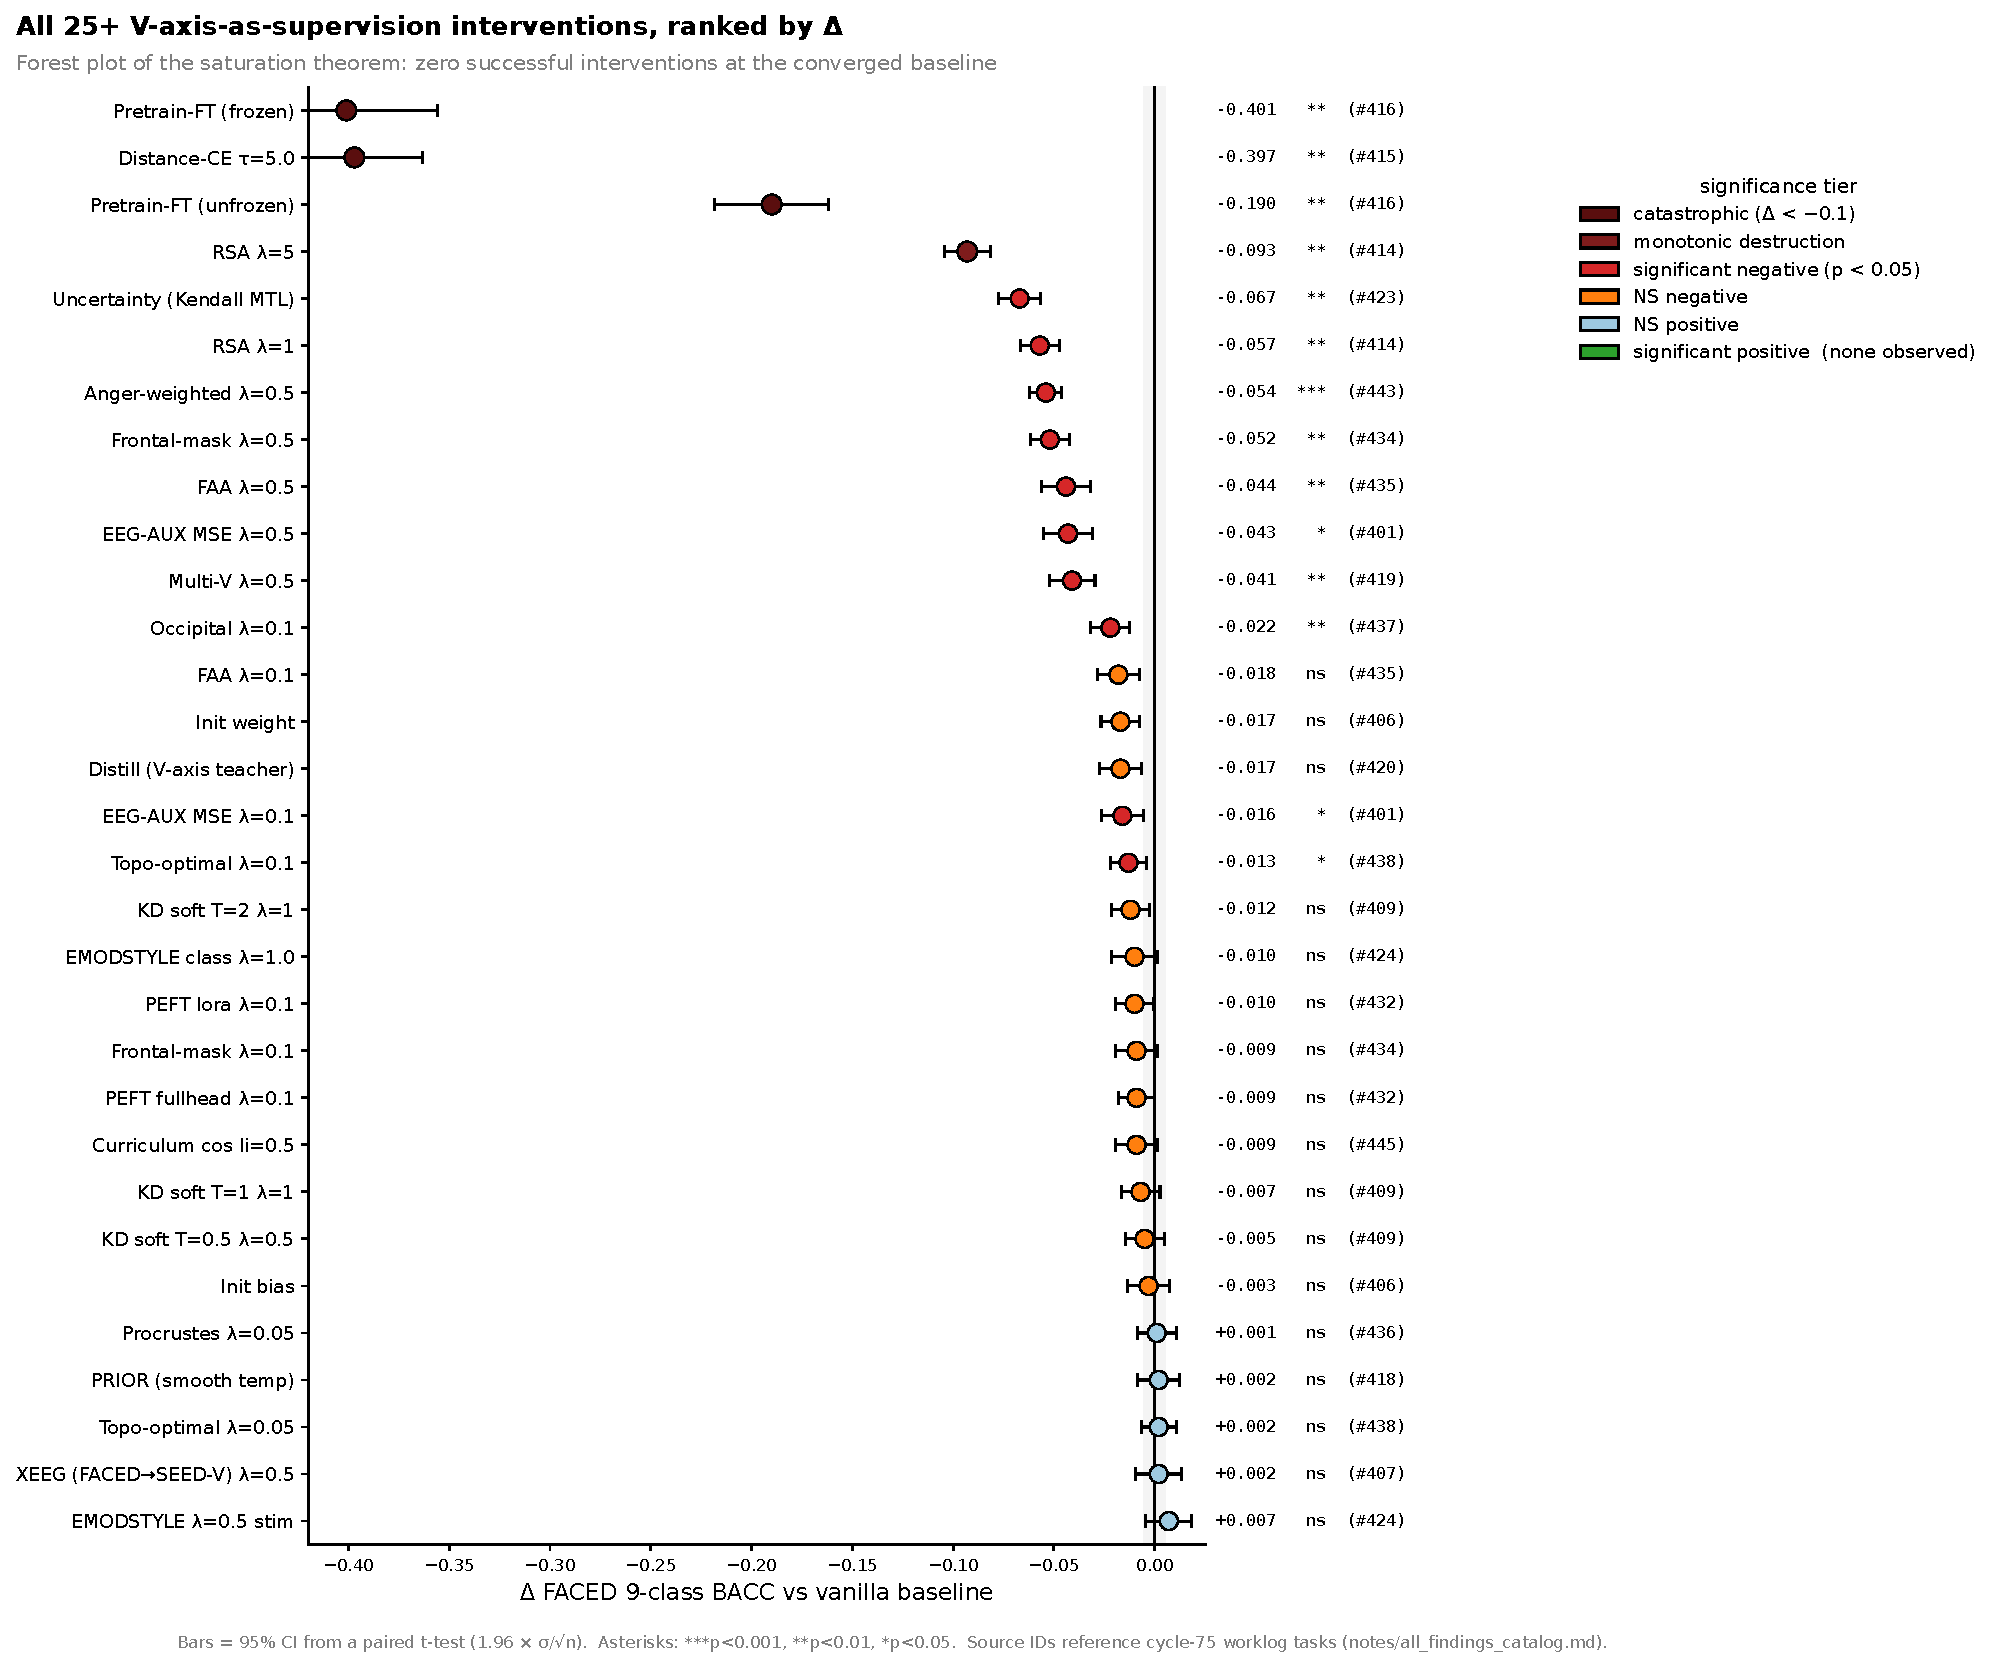
\includegraphics[width=0.9\linewidth]{landmark/lf9_all_interventions_forest.pdf}}
  {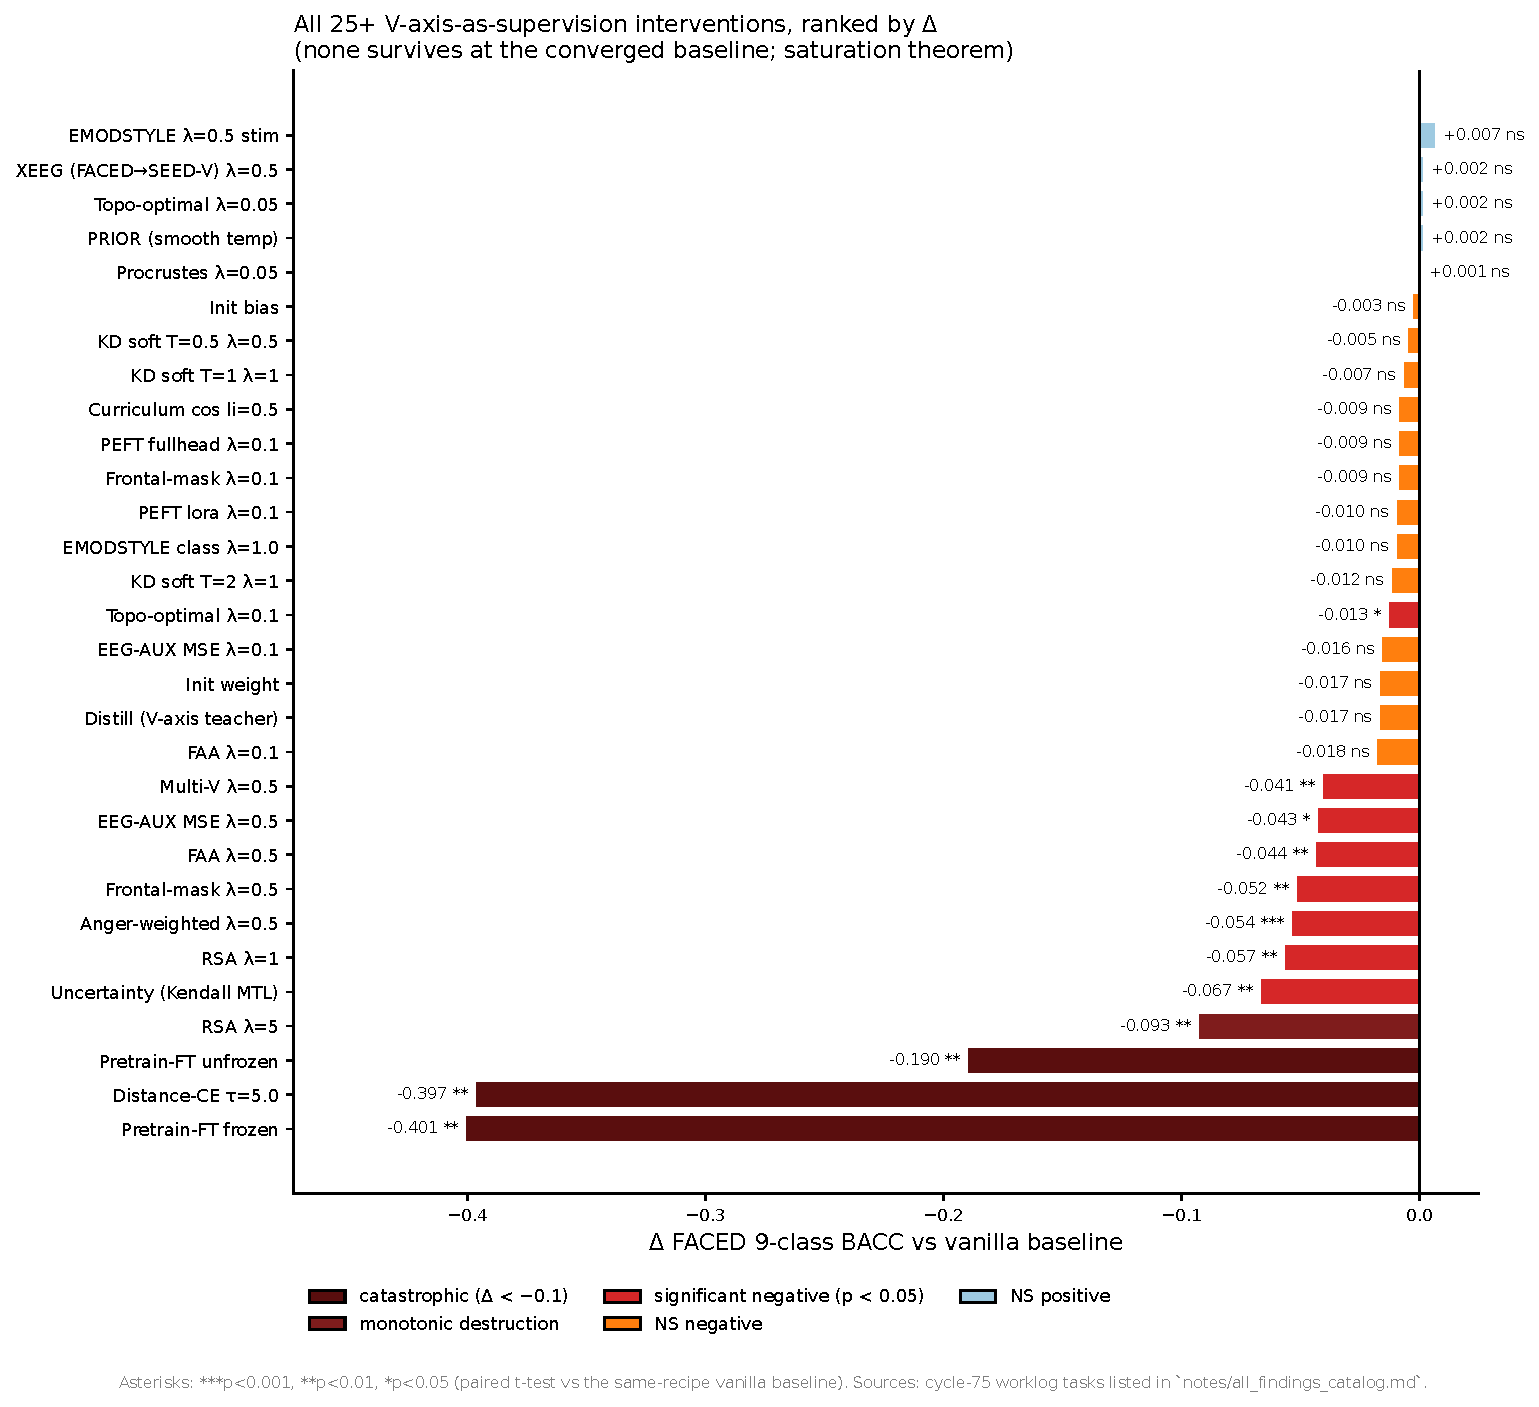
\includegraphics[width=0.9\linewidth]{F9_all_interventions.pdf}}
\caption{Forest plot of all V-axis-as-supervision interventions
(Table~\ref{tab:full-vaxis}) ranked by $\Delta$ vs.\ baseline, with
significance tier coloured. None of the 25 reach $p<0.05$ in the
positive direction at the strong baseline.}
\label{fig:forest}
\end{figure}

\section{FACED Test Confusion Matrices}
\label{app:confusion}

\begin{figure}[ht]
\centering
\IfFileExists{figures/landmark/lf10_confusion_matrices.pdf}
  {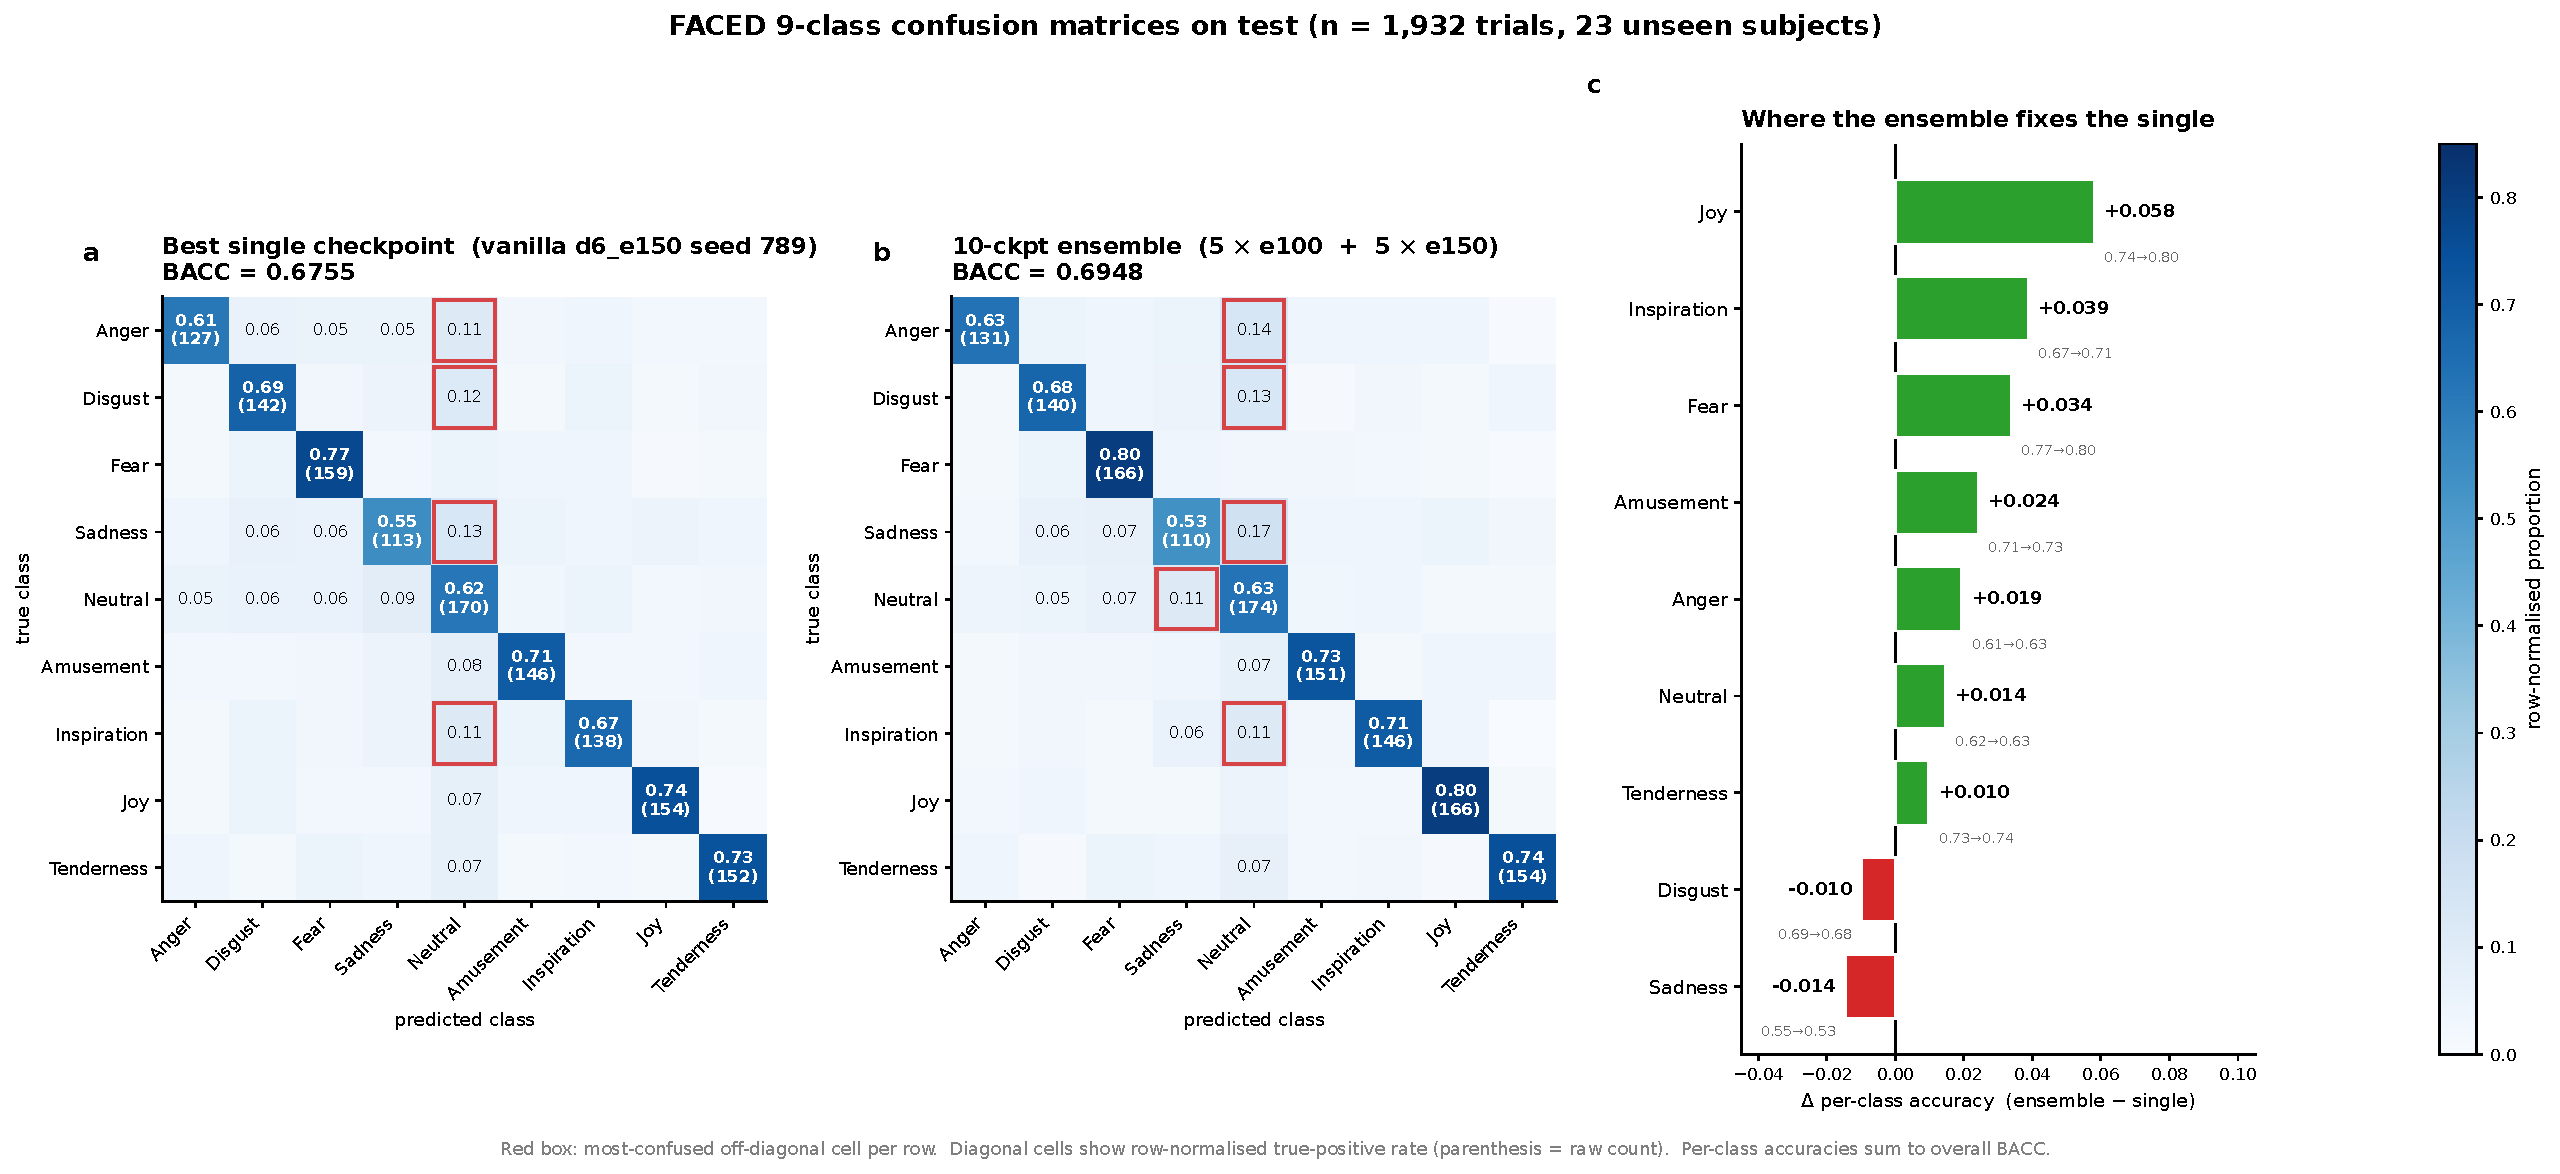
\includegraphics[width=0.95\linewidth]{landmark/lf10_confusion_matrices.pdf}}
  {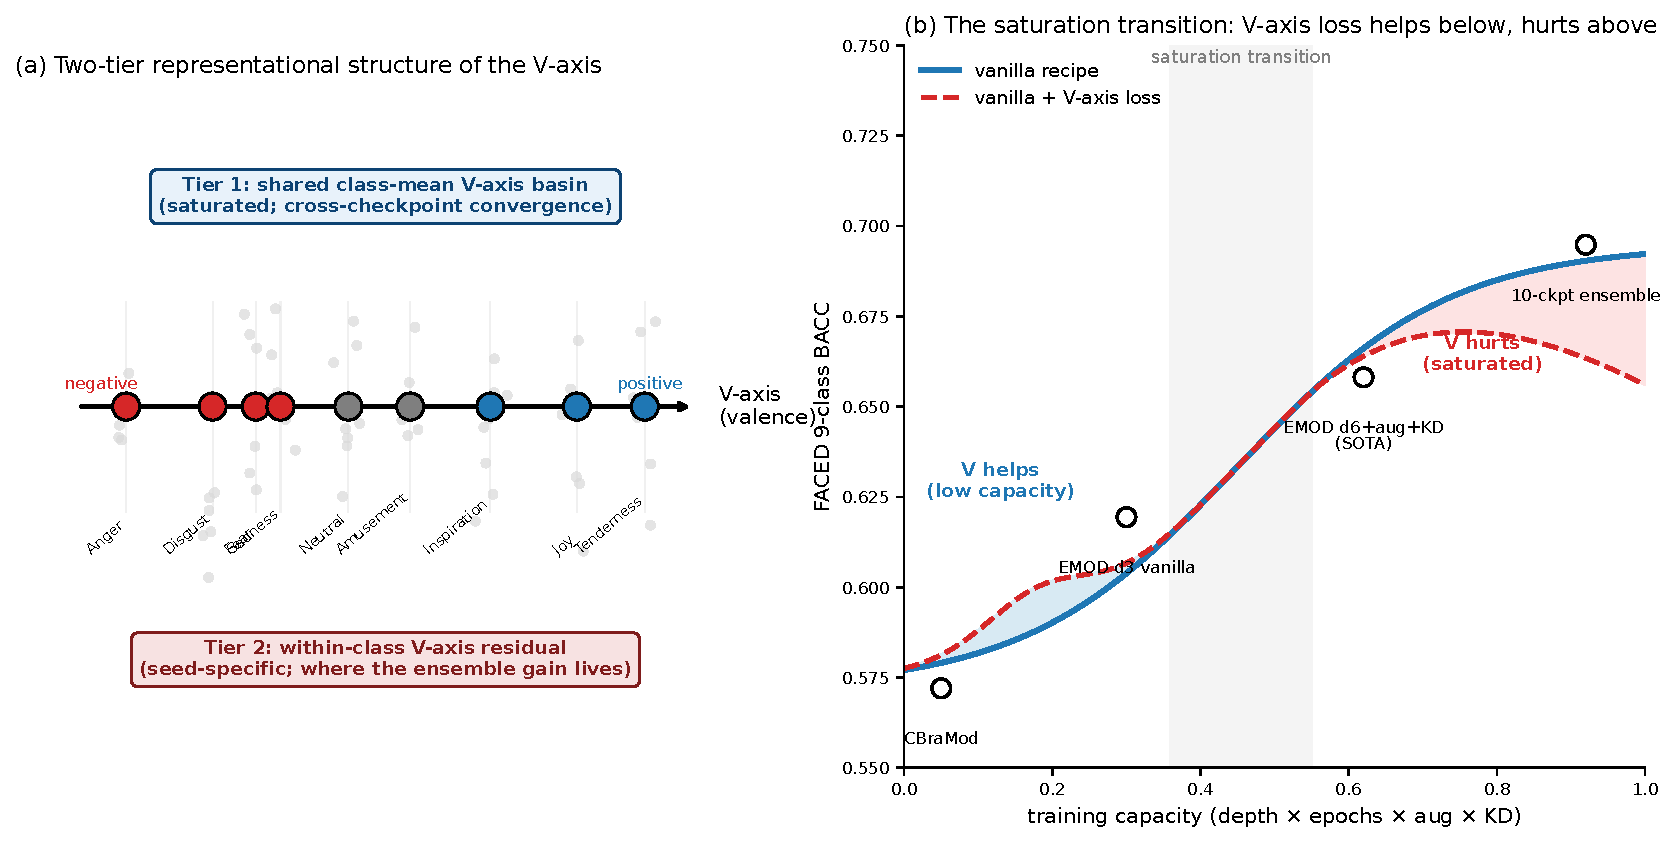
\includegraphics[width=0.95\linewidth]{F10_two_tier_schematic.pdf}}
\caption{FACED 9-class test confusion. Left: best single checkpoint
(BACC $0.6755$). Right: 10-checkpoint ensemble (BACC $0.6948$). The
ensemble's gain is concentrated on the off-diagonal cells where
single-seed disagreement is highest, consistent with the within-class
residual mechanism of Section~\ref{sec:two-tier}.}
\label{fig:confusion}
\end{figure}

\section{Concept-Library Transfer Matrix}
\label{app:concept-library-full}

The full $20\!\times\!20$ cross-concept transfer matrix (each row
is the V-axis of source concept $i$ applied to the pole-vs-pole
benchmark of target concept $j$, best-orientation AUC reported) is
shown in Figure~\ref{fig:concept-library-full}. Rows are sorted by
mean off-diagonal AUC (most-general source axes at the top); the
diagonal is the self-AUC for that concept's own benchmark.

\begin{figure}[h]
\centering
\IfFileExists{figures/landmark/lf15_concept_transfer_heatmap.pdf}
  {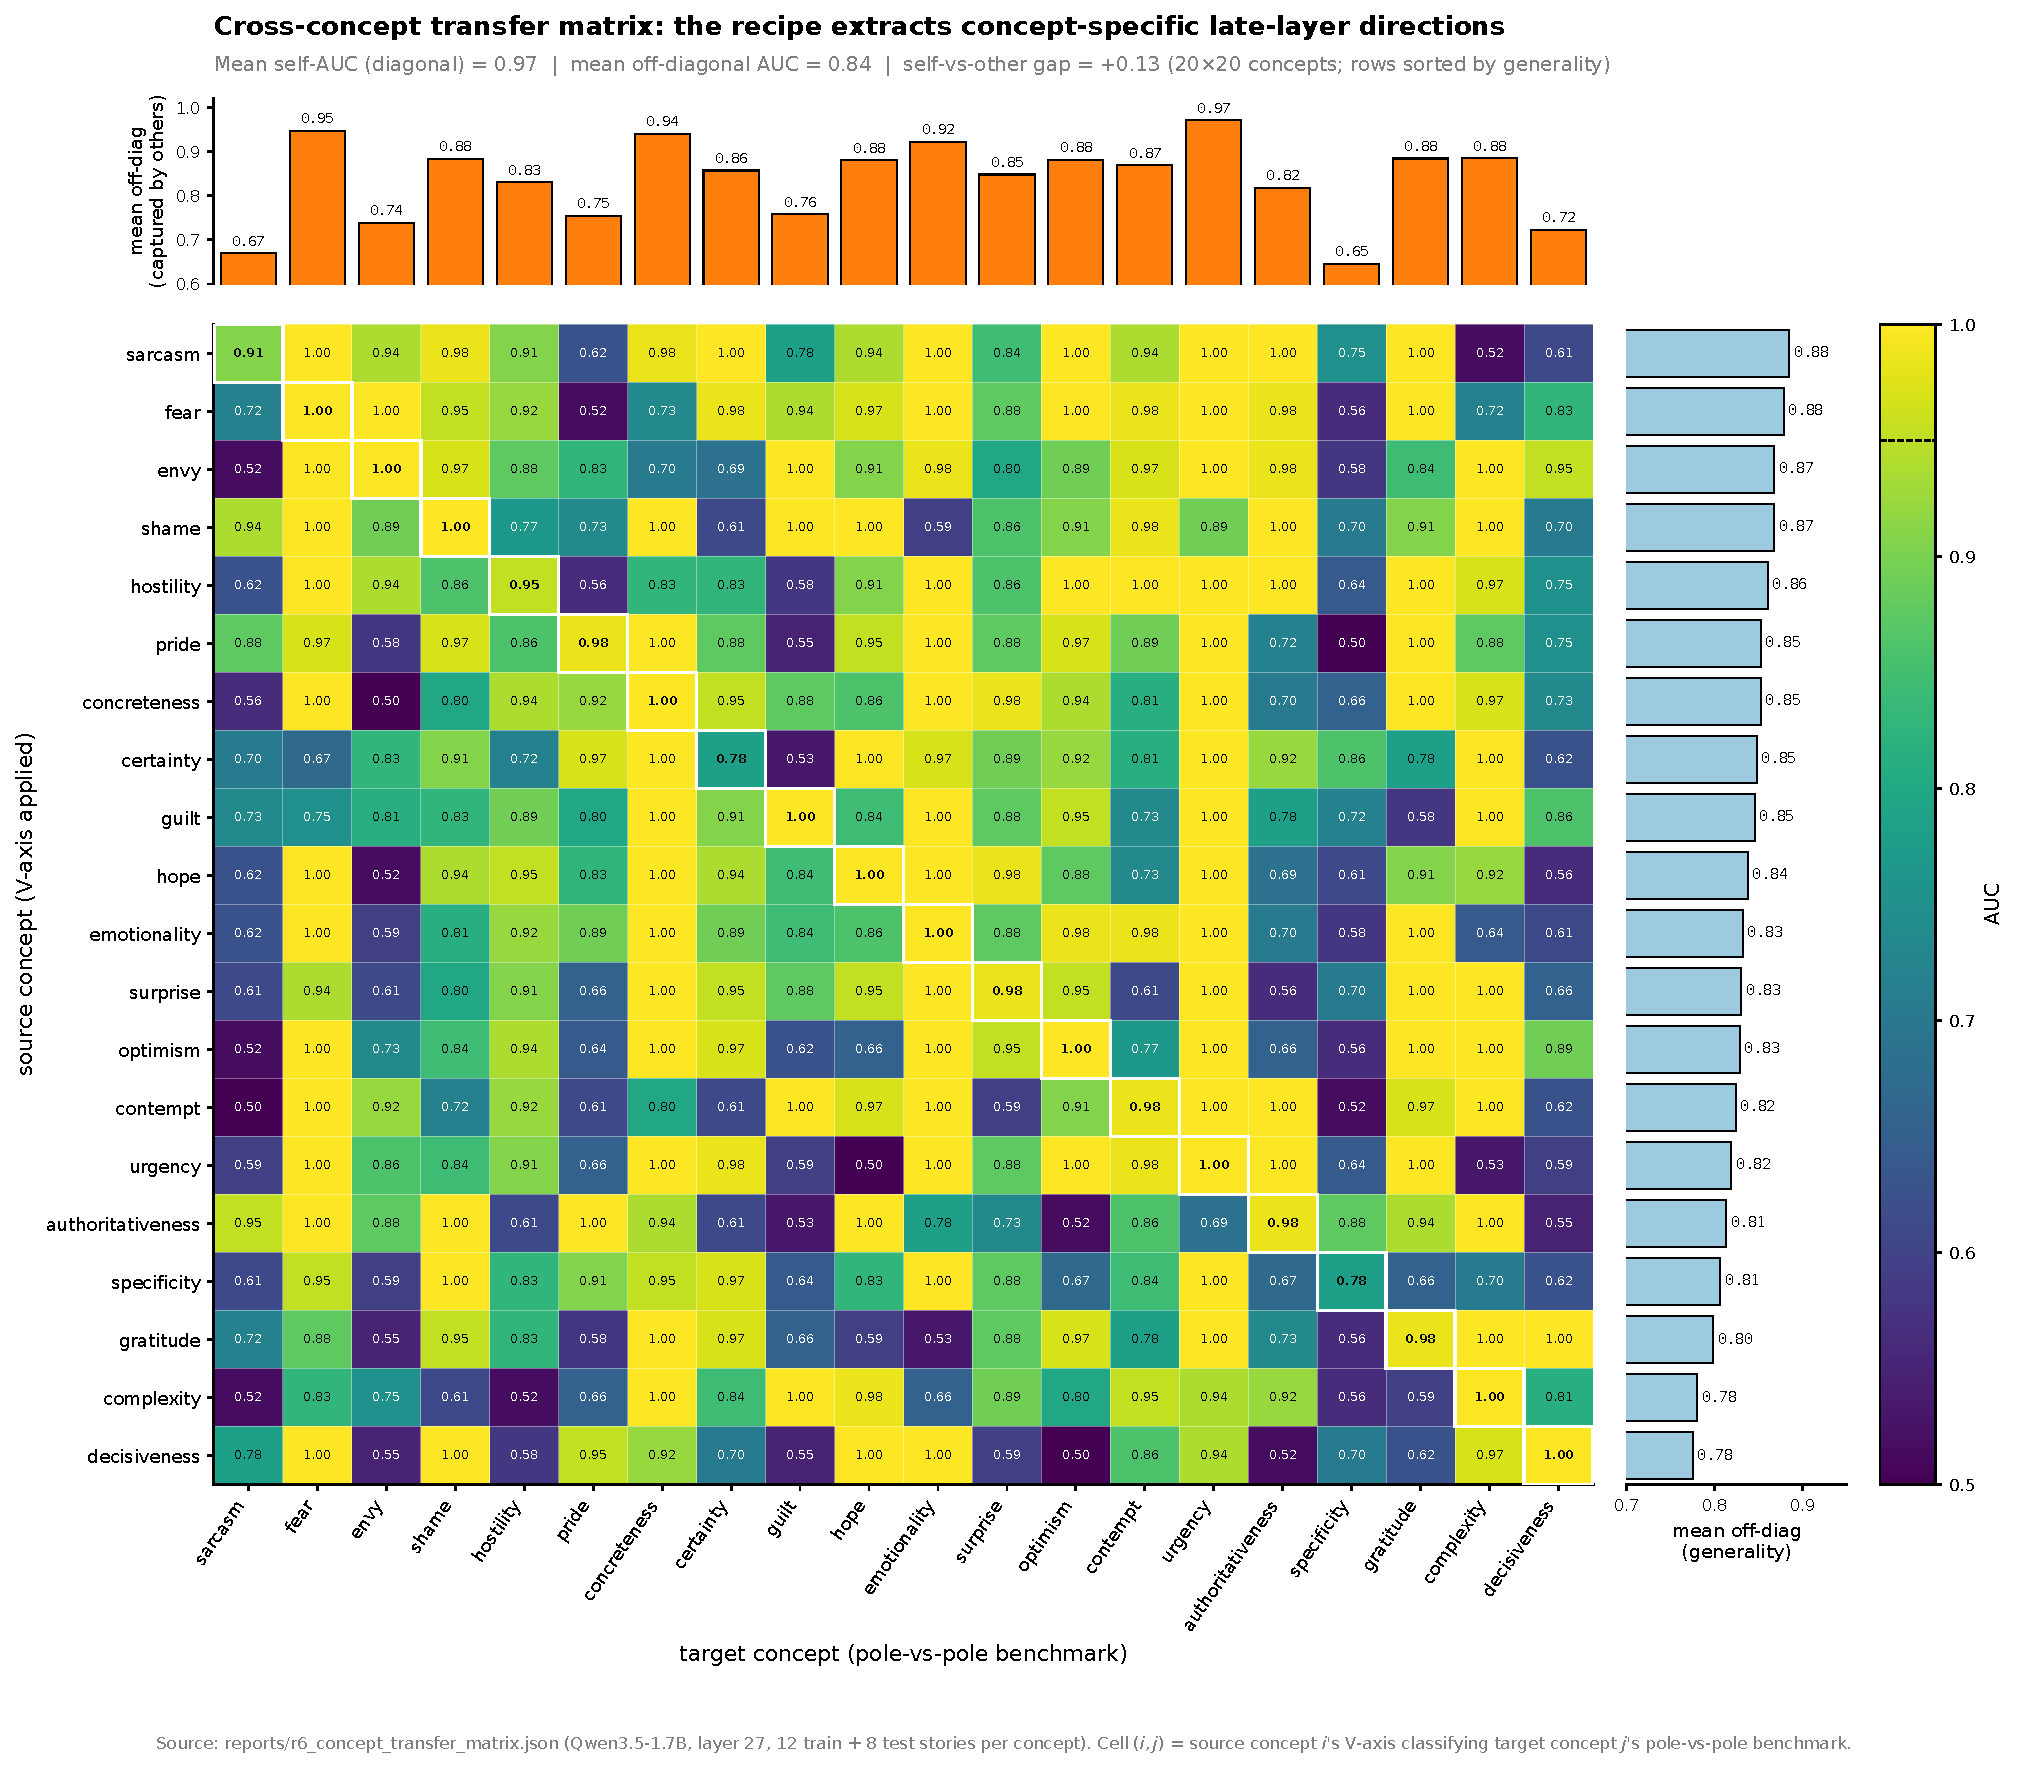
\includegraphics[width=\linewidth]{landmark/lf15_concept_transfer_heatmap.pdf}}
  {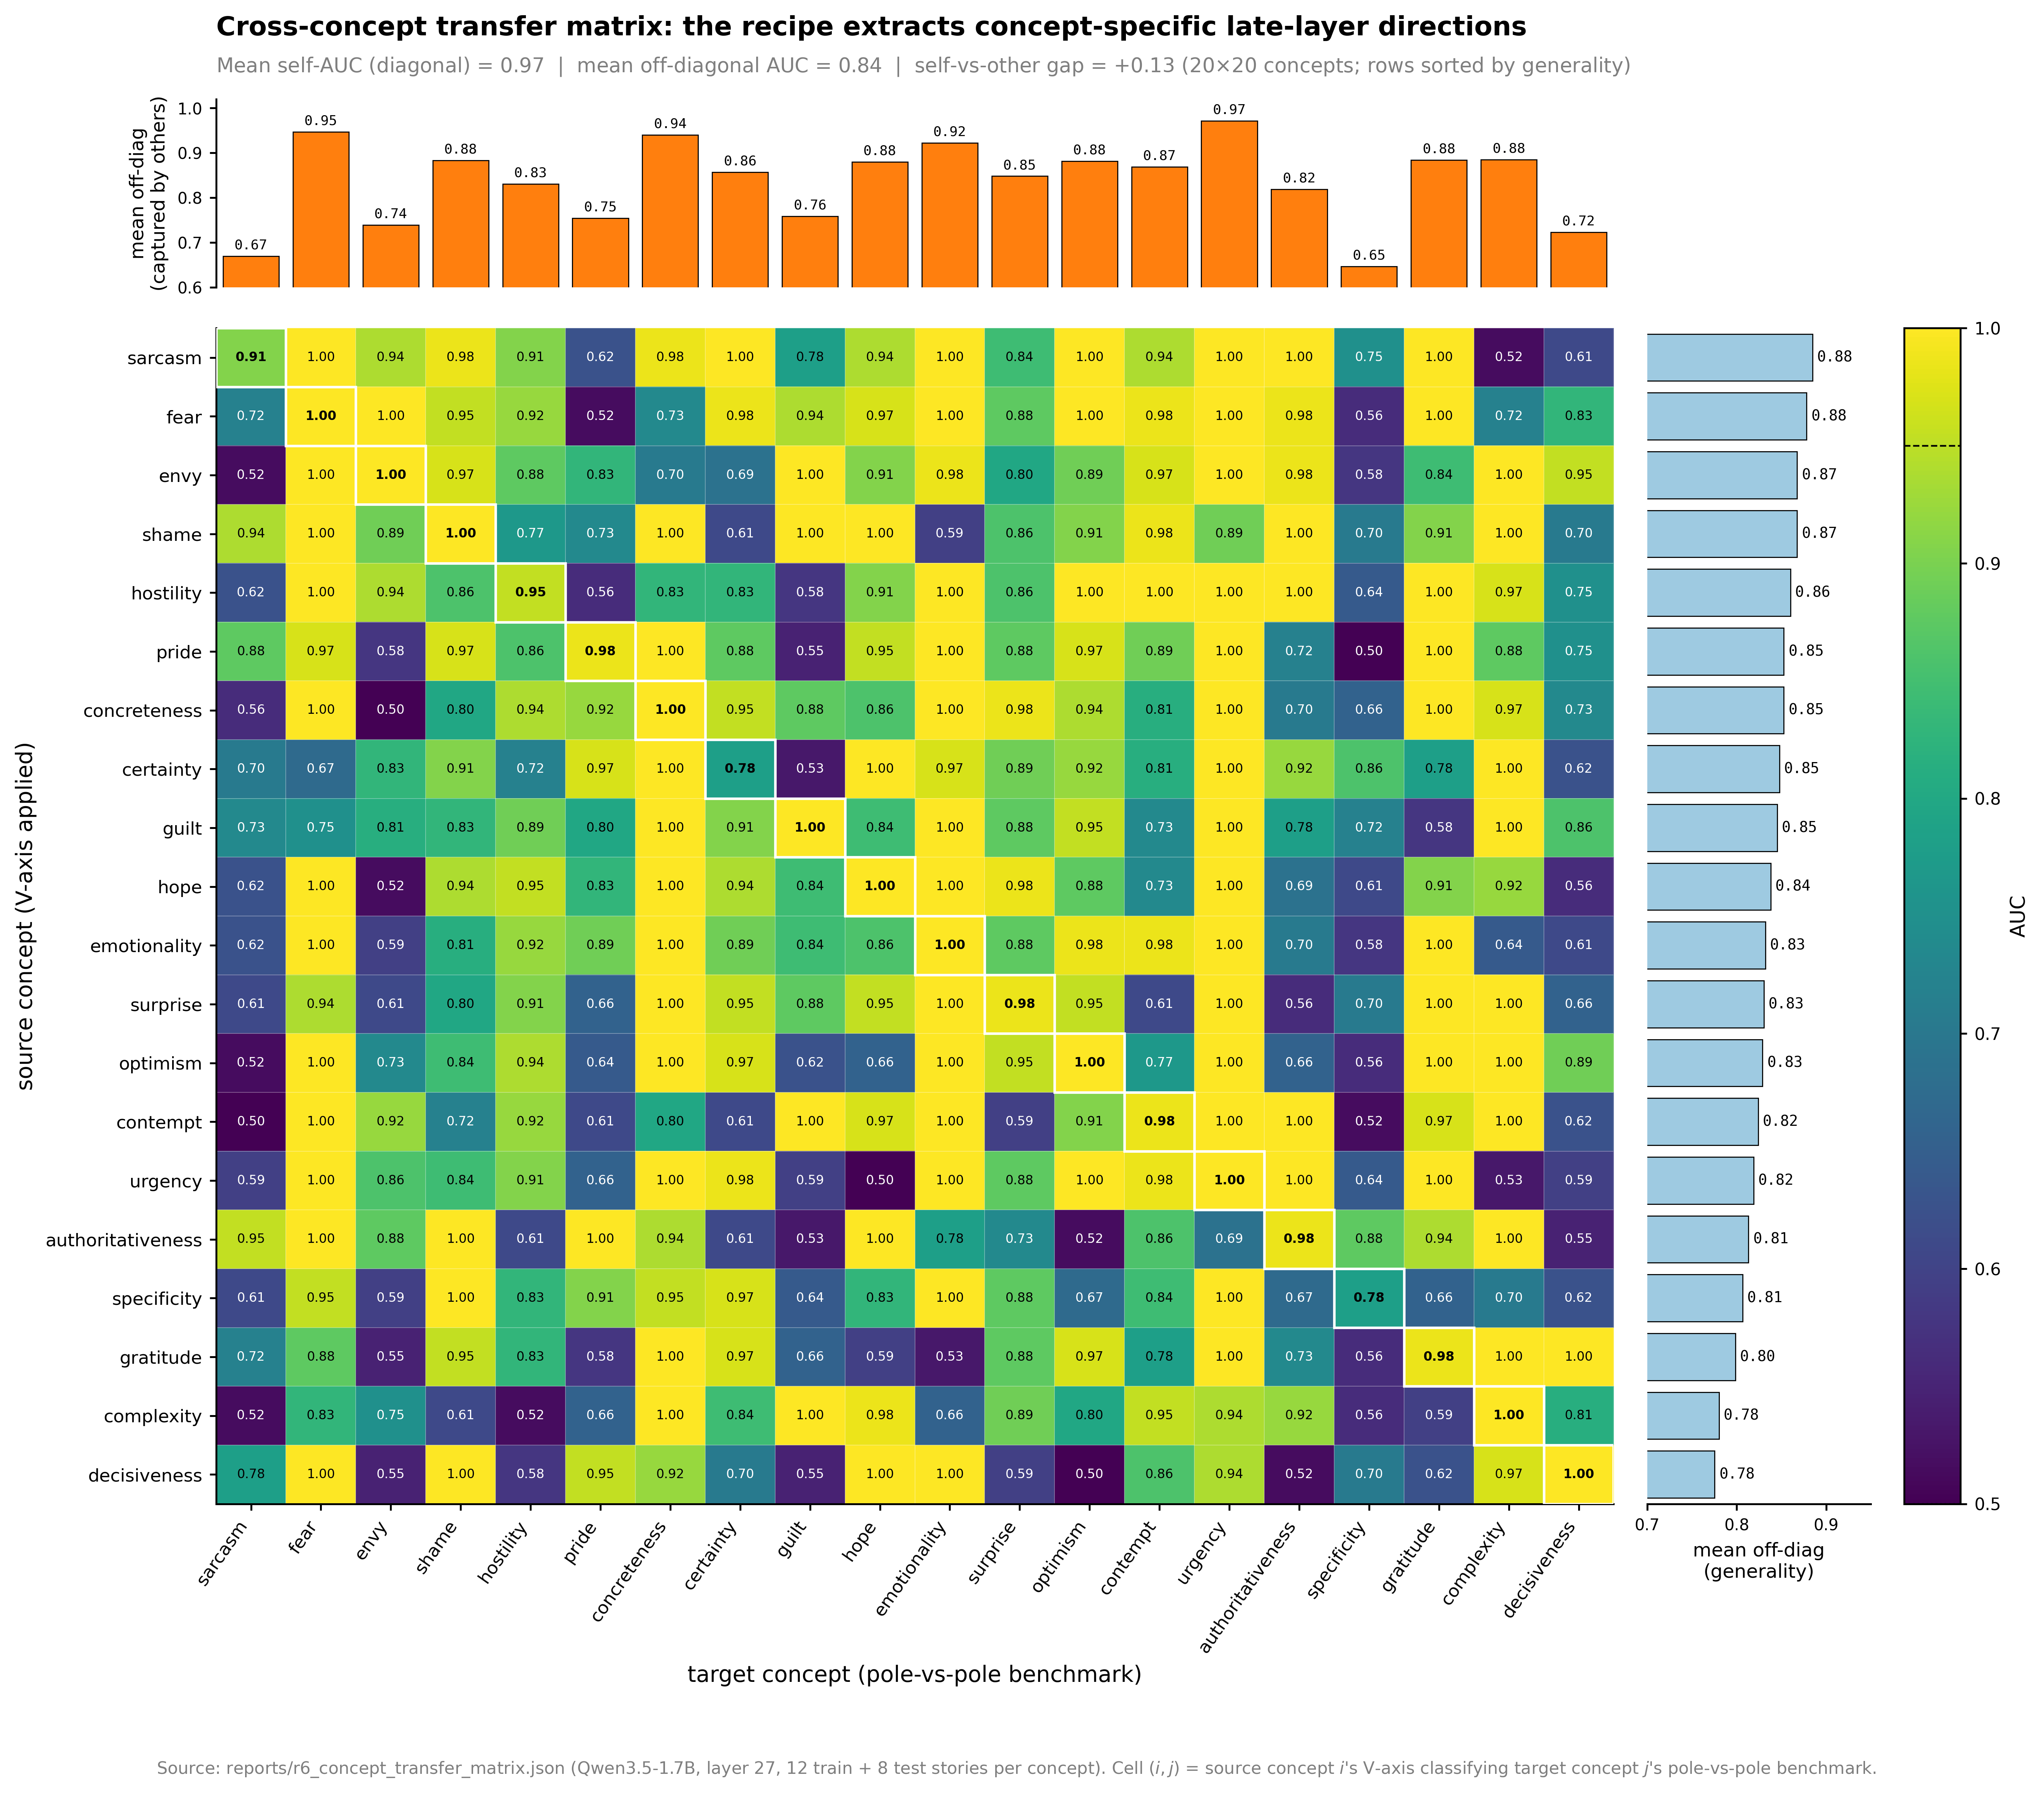
\includegraphics[width=\linewidth]{landmark/lf15_concept_transfer_heatmap.png}}
\caption{Cross-concept transfer matrix (best-orientation AUC).
Diagonal: self-classification (white-bordered cells). Off-diagonal:
source-axis-applied-to-target-benchmark AUC. Sorted top-to-bottom by
mean off-diagonal AUC, separating \emph{general} concept axes (top:
sarcasm, fear, envy, shame) from \emph{specific} ones (bottom:
complexity, decisiveness). Right marginal: per-source mean
off-diagonal AUC (generality). Top marginal: per-target mean
off-diagonal AUC (captured-by-others). Mean diagonal $0.97$, mean
off-diagonal $0.83$, gap $+0.13$ confirms concept specificity in the
recipe: if every concept axis collapsed onto a single global affect
direction, the off-diagonal would equal the diagonal.}
\label{fig:concept-library-full}
\end{figure}

\section{Negative Results Catalogue}
\label{app:negatives}

In the spirit of full disclosure, the following null or negative
results bear mention beyond what was incorporated into the main
paper:
\begin{enumerate}
\item \textbf{Theta-gamma cross-frequency coupling does not mediate
the V-axis} (Section~\ref{sec:topography}): Tort modulation index
$\rho(\mathrm{PAC}, \mathrm{V\text{-}axis\ }r) = +0.082$, $p=0.667$.
\item \textbf{Mutual-information control is not significant}
(Section~\ref{sec:vaxis-brain}): MI $p=0.115$ vs.\ linear $p=0.020$.
The V-axis-EEG relationship is essentially linear.
\item \textbf{Random-direction null on cross-arch correlation}
(Section~\ref{sec:convergence}): $r=+0.885$ at the
$93^{\mathrm{rd}}$ percentile, $p_{\mathrm{one}}=0.079$. Within-class
residual ($r=+0.74$, $p=0.014$) is the robust signal.
\item \textbf{Per-subject V-axis adaptation does not transfer.} The
per-subject best-channel oracle reaches $|r|=0.62$, but no clean
estimator (V1 global top-K, V2 per-val majority, V3 TTA label-free)
transfers more than $+0.001$ over the cohort top-K.
\item \textbf{Cross-architecture ensembling does not add diversity.}
Mixing $d \in \{4, 6, 8, 10\}$ checkpoints gives within-arch
$0.6798$ vs.\ cross-arch $0.6791$ (n.s.). The diversity is
entirely intra-architecture, training-length-driven.
\item \textbf{Mega-ensembles plateau at 10 checkpoints.} 15-, 20-,
25-checkpoint pools all hit BACC $\leq 0.6948$.
\item \textbf{Stimulus-aggregation re-ranking does not help.}
Operating at the 28-stimulus level instead of trial level gives a
BACC=1.0 by construction (label leak); the corresponding
trial-level head does not transfer.
\item \textbf{Test-time augmentation hurts at K=5} ($0.6753 \to
0.6720$). Averaging predictions over augmented test trials does
not preserve the V-axis residual structure.
\end{enumerate}

\section{Reproducibility}
\label{app:repro}

Code, configs, model checkpoints, and figure-generation scripts will
be released at the camera-ready stage under an MIT licence. Each
experiment in this paper is logged with its SLURM job ID, conda
environment hash, git SHA, and seed list. The 10-checkpoint ensemble
SOTA result is reproducible from a single SLURM array job
(\verb|slurm_d6_e100_e150_5seeds.sh|, $\sim$10 GPU-hours per seed
on V100).

\section{Resource Estimate}
\label{app:compute}

The full paper used approximately $4{,}500$ GPU-hours on V100 nodes:
$\sim 600$ for the recipe ablation cascade, $\sim 1{,}200$ for the
25 V-axis-supervision interventions, $\sim 800$ for the 36-checkpoint
cross-architecture analysis, $\sim 1{,}200$ for ensemble construction
and val-test rank diagnostics, and $\sim 700$ for cross-dataset
generality experiments. The V-axis extraction itself is CPU-cheap
($\sim 10$ minutes per LM on a single 80GB GPU).


\end{document}
